\section{Rete neurale}
\label{Rete neurale}

La libreria utilizzata per sviluppare la Rete neurale \`e stata \textit{ConvNetJS}. L'aspetto positivo di tale scelta \`e stata la semplicit\`a nell'utilizzo del linguaggio javascript; l'aspetto negativo ha riguardato la totale mancanza di mantenibilit\`a della libreria stessa che comporta la scarsit\`a di esempi applicativi, oltre alla documentazione ufficiale, che costringono lo sviluppatore ad una ricerca approfondita personale in un ambiente ove lo nozioni si presentano scarse e a continue prove per verificare la validit\`a del codice prodotto.
\begin{figure}[H]
\centering
	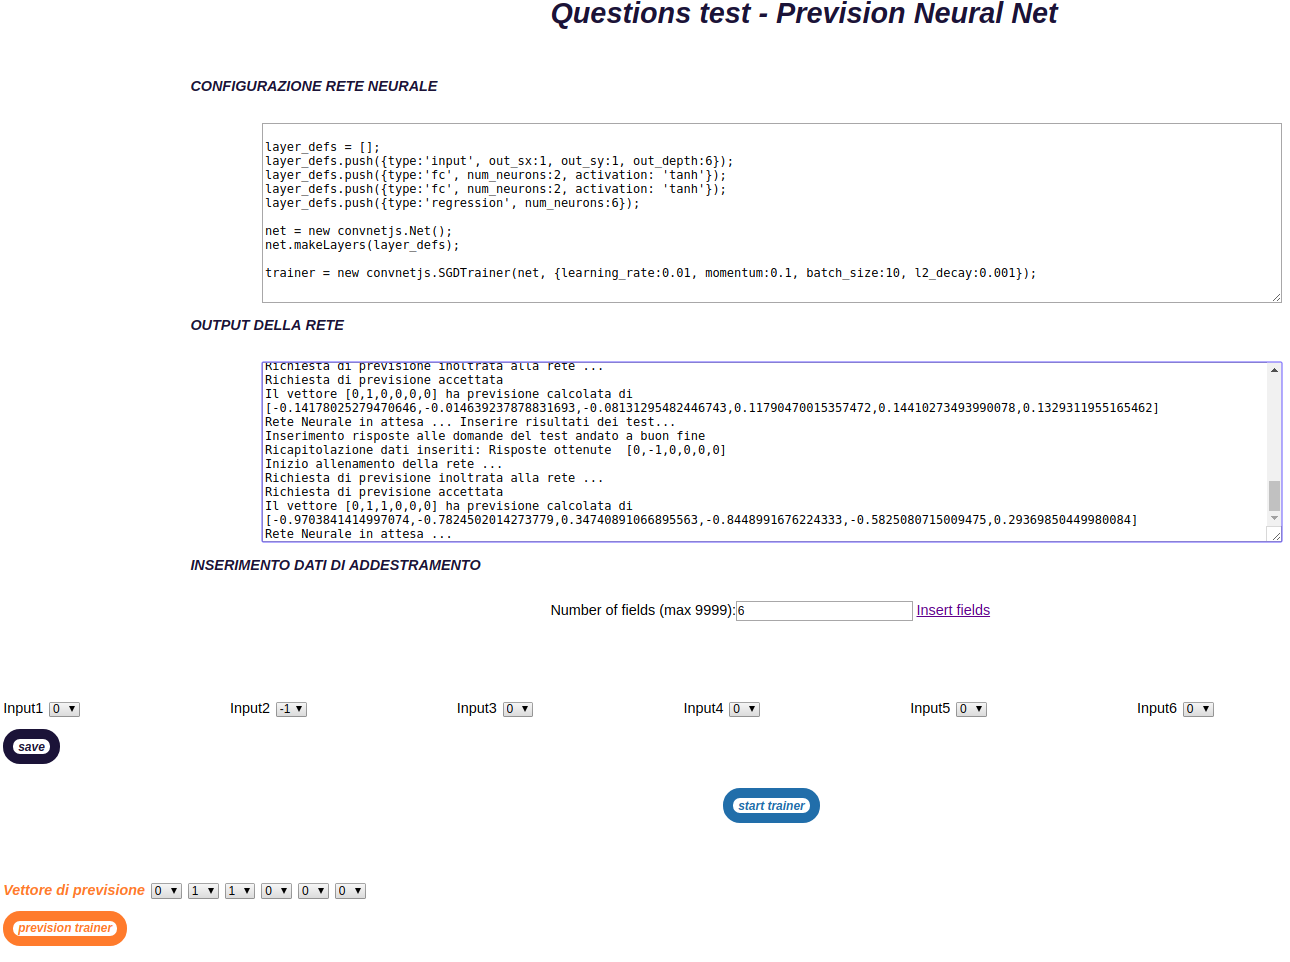
\includegraphics[width=1\linewidth]{./image/GUI-rete-neurale.png}
	\caption{Interfaccia utente della Rete neurale di prova.}
	\label{Interfaccia utente della Rete neurale di prova.}
\end{figure}
\noindent
Durante il periodo 24/05 - 31/05 mi sono occupata dello sviluppo di una Rete neurale in grado di ricevere in input un training set di dimensione 6 e di restituire una previsione sui dati di apprendimento ricevuti.
\noindent
Il problema che la rete mira ad analizzare \`e quello discusso nel precedente capitolo \textit{Analisi dei dati di probabilit\`a}
\\\\
Per agevolare l'apprendimento della rete, ed ottenere delle previsioni stabili mi sono occupata di implementare due metodi di generazione randomica di dati in modo da far apprendere massicciamente la stessa.
Il dato prodotto consiste in un vettore di 6 elementi, composto da  -1, 0 e 1 con il seguente criterio:
\begin{itemize}
\item \textbf{-1}: la domanda x \`e stata posta al candidato che ha risposto in maniera errata;
\item \textbf{0}: la domanda x non \`e stata posta al candidato;
\item \textbf{1}: la domanda x \`e stata posta al candidato che ha saputo rispondere correttamente.
\end{itemize}
\noindent
Il primo metodo che ho sviluppato si occupa di generare un vettore di dati di apprendimento basandosi esclusivamente su come le domande sono interconnesse tra di loro (grazie all'uso di un grafo della conoscenza costruito ad hoc); il secondo metodo ripropone quanto perseguito dal primo metodo con il valore aggiunto di generazione di un profilo randomico di un candidato, che tiene conto della  probabilit\`a di risposta ad una domande seguendo la formula P(A)= $\frac{1}{3}+\frac{1}{6}P(S_1)+\frac{2}{3}P(S_2)$.

\subsection{Test effettuati}
\label{Test effettuati}

Alcune decisioni che ho preso durante la scelta dell'architettura della rete riguardano i seguenti settori:
\begin{enumerate}
\item Una rete neurale non deve, per fornire dei dati attendibili, possedere un numero di neuroni troppo elevato rispetto al trainset effettuato; altrimenti la previsione  ritornerebbe l'identit\`a del vettore di input della stessa, come conseguenza diretta della capacit\`a troppo elevata di immagazzinare dati.
\item I layers, ho deciso, di allenarli mediante tecnica di regressione, che permette l'inserimento in input di una funzione obiettivo e l'ottenimento di un risultato, in output, anche in virgola mobile e composto di tanti elementi quanti sono i neuroni di regressione dichiarati. Per la mia rete di prova \`e necessario dichiarare  6 neuroni in regressione perch\`e l'output, appunto, che ci si aspetta dal sistema \`e di 6 elementi.
\item Per costruire un dataset di dati consistente che permettesse alla rete di imparare qualcosa ho costruito un grafo della conoscenza con lo scopo di mettere in relazione degli argomenti che coinvolgono uno o pi\`u domande.
\begin{figure}[H]
\centering
	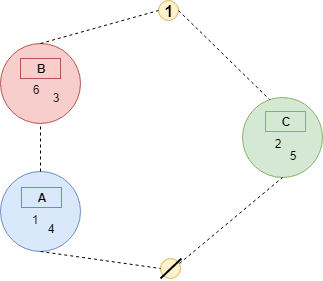
\includegraphics[width=0.60\linewidth]{./image/grafo_trainset.png}
	\caption{Grafo rappresentante le relazioni esistenti tra il set di domande di prova.}
	\label{Grafo rappresentante le relazioni esistenti tra il set di domande di prova.}
\end{figure}
\noindent
Per svolgere l'apprendimento ogni vettore, facente parte del dataset, viene dato in pasto alla rete che a sua volta provvede alla sua assimilazione come conoscenza mediante la tecnica dell'autoencoder, ovvero la rete impara il vettore riducendone lo spazio occupato.
\item Per creare il dataset ho ritenuto sufficiente generare \textit{2000} vettori di risposta in modo da compiere in maniera esaustivo l'apprendimento della rete.
\end{enumerate}
\noindent
Il vettore passato in input per svolgere le previsioni \`e \textit{[0,0,0,0,0,0]},\textit{[0,0,1,0,1,0]} e \textit{[0,0,-1,0,0,0]}\\
Le aspettative riguardano la previsione di risposta di un candidato
\noindent. 
Di seguito riporto quanto \`e stato rilevato in fase di test.

\subsubsection{Architettura  della rete: 4 neuroni per ciascuno dei 2 layers}
\label{Configurazione della rete: 4 neuroni per ciascuno dei 2 layers}

Architettura  della rete utilizzata:\\
\begin{verbatim}layer_defs = [];
layer_defs.push({type:'input', out_sx:1, out_sy:1, out_depth:6});
layer_defs.push({type:'fc', num_neurons:4, activation: 'tanh'});
layer_defs.push({type:'fc', num_neurons:4, activation: 'tanh'});
layer_defs.push({type:'regression', num_neurons:6});

net = new convnetjs.Net();
net.makeLayers(layer_defs);

trainer = new convnetjs.SGDTrainer(net, {learning_rate:0.01,
 momentum:0.1, batch_size:10, l2_decay:0.001});
\end{verbatim}
\noindent
I layers utilizzati sono 2 e compositi da 4 neuroni.

\paragraph{Training set standard a 4 neuroni per ciascuno dei 2 layers}\mbox{}
\label{Training set standard a 4 neuroni per ciascuno dei 2 layers}
\\
\noindent
\begin{itemize}
\item \begin{verbatim}Il vettore [0,0,0,0,0,0] ha previsione calcolata di
[-0.021598804903572744,-0.1372509042342871,0.06611969158456255,
0.018121335417653706,-0.11264571886853292,0.17520370837747462]\end{verbatim}
Appaiono in relazione le domande 1, 2, 5 e 3, 4, 6.\\
Gli scostamenti tra le coppie 2, 5 e 3, 6 sono consistenti con quelle che sono le relazioni di dipendenza, invece 1, 4 ha una differenza di 0.016 circa che parte da qualche millesimo fino 0.5
Le domande 3 e 6 si dovrebbero presentare con una positivit\`a inferiore rispetto a 1 e 4; nel test in analisi questo non viene rispettato da nessuna delle coppie in analisi per differenze che vanno da qualche millesimo fino a 0.018 circa.
\paragraph{Osservazioni}\mbox{}
\label{Osservazioni su rete a 4 neuroni per ciascuno dei 2 layers}
\\\\
\noindent
L'architettura testata si compone di 4 neuroni a layer su una base di 2000 test correndo il rischio di avere una rete che apprende troppo e come effetto negativo "veda" addirittura cose che non esistono. A prova di ci\`o sono i risultati non conformi alle attese.
Dunque mi fermo qui con il test di tale architettura e riducendone il numero di neuroni presenti in ciascun layers e/o il numero di layers presenti.\\

Le nuove architetture su cui ho effettuato i test sono esposte nei paragrafi seguenti.

\subsubsection{Architettura della rete a 2 neuroni per ciascuno dei 2 layers}
\label{Architettura della rete a 2 neuroni per ciascuno dei 2 layers}
Architettura  della rete utilizzata:\\
\begin{verbatim}layer_defs = [];
layer_defs.push({type:'input', out_sx:1, out_sy:1, out_depth:6});
layer_defs.push({type:'fc', num_neurons:2, activation: 'tanh'});
layer_defs.push({type:'fc', num_neurons:2, activation: 'tanh'});
layer_defs.push({type:'regression', num_neurons:6});

net = new convnetjs.Net();
net.makeLayers(layer_defs);

trainer = new convnetjs.SGDTrainer(net, {learning_rate:0.01,
 momentum:0.1, batch_size:10, l2_decay:0.001});
\end{verbatim}
\noindent
I layers utilizzati sono 2 compositi da 2 neuroni.

\paragraph{Training set standard su rete a 2 neuroni per ciascuno dei 2 layers}\mbox{}
\label{Training set standard su rete a 2 neuroni per ciascuno dei 2 layers}
\\
\noindent
\begin{itemize}
\item \begin{verbatim}[Il vettore [0,0,0,0,0,0] ha previsione calcolata di
[0.31232372051574936,0.7253754889487585,-0.5051208979797573,
0.32075742158673093,0.7324947496336937,-0.4348299972940168]
\end{verbatim}
Appaiono in relazione le domande 1, 2, 4, 5 e 3, 6.\\
Gli scostamenti tra le coppie 1, 4 e 3, 6  e 2, 5 sono consistenti con quelle che sono le relazioni di dipendenza fra le domande.
Le domande 3 e 6 si dovrebbero presentare con una positivit\`a inferiore rispetto a 1 e 4; in questo test la regola viene rispettata pienamente.\\
Dai dati della previsione si nota come il candidato ha una buona probabilit\`a di saper rispondere alla coppia 1 e 4, e ancora pi\`u elevata di saper rispondere correttamente alla coppia 2 e 5; molto bassa di saper rispondere correttamente alle 3 e 6 che sono, appunto, di una difficolt\`a maggiore rispetto alla coppia 1 e 4.

\item \begin{verbatim}Il vettore [0,0,1,0,1,0] ha previsione calcolata di
[0.5123144717131076,0.9123354449531641,0.2837937822420923,
0.46449868699771607,0.9029832167165894,0.3227303792035435]
\end{verbatim}
Appaiono in relazione le domande 1, 2, 3  4, 5, 6.\\
Gli scostamenti tra le coppie 1, 4 e 3, 6  e 2, 5 sono consistenti con quelle che sono le relazioni di dipendenza fra le domande.
Le domande 3 e 6 si dovrebbero presentare con una positivit\`a inferiore rispetto a 1 e 4; in questo test la regola viene rispettata pienamente.\\
Dai dati della previsione si nota come il candidato ha un'ottima probabilit\`a di saper rispondere alla coppia 2 e 5 (come imposto dal vettore previsione), buona di saper rispondere alla coppie 3 e 6 (come imposto dal vettore previsione) e pi\`u che buona  di saper rispondere alle 1 e 4, che sono di una semplicit\`a pi\`u elevata rispetto alla 3 e 4.
\end{itemize}

\item \begin{verbatim}Il vettore [0,0,-1,0,0,0] ha previsione calcolata di
[0.3698539826215957,0.288907514487717,-0.8504159455662308,
0.3663192502433841,0.2937448801761998,-0.7845589473185985]
\end{verbatim}
Appaiono in relazione le domande 1, 2, 4, 5 e 3, 6.\\
Gli scostamenti tra le coppie 1, 4 e 3, 6  e 2, 5 sono consistenti con quelle che sono le relazioni di dipendenza fra le domande.
Le domande 3 e 6 si dovrebbero presentare con una positivit\`a inferiore rispetto a 1 e 4; in questo test la regola viene rispettata pienamente.\\
Dai dati della previsione si nota come il candidato ha una discreta probabilit\`a di saper rispondere alla coppia 2 e 5, un p\`o meglio di saper rispondere alla coppie 1 e 4 e pi\`u di non saper saper rispondere alle 3 e 6 (come imposto dal vettore previsione).
\end{itemize}

\paragraph{Training set con generazione del profilo di un candidato e calcolo delle probabilit\`a di risposta a 2 neuroni per ciascuno dei 2 layers}\mbox{}
\label{Training set con generazione del profilo di un candidato e calcolo delle probabilita di risposta a 2 neuroni per ciascuno dei 2 layers}
\\
\noindent
\begin{itemize}
\item \begin{verbatim}Il vettore [0,0,0,0,0,0] ha previsione calcolata di
[0.057781303506280995,0.0513731100126314,-0.06600467867066256,
0.029940883111932555,-0.019564515397168573,-0.09570617900597932]
\end{verbatim}
Appaiono in relazione le domande 1, 2, 4 e 3, 5, 6.\\
Gli scostamenti tra la coppia 1, 4 e 3, 6 sono consistenti con  quelle che sono le relazioni di dipendenza fra le domande; invece per la coppia 2 e 5 i segni sono opposti con una differenza di 0.024.
Le domande 3 e 6 si dovrebbero presentare con una positivit\`a inferiore rispetto a 1 e 4, la regola viene rispettata pienamente. Le anomalie riscontrate sono da ricondurre alla natura del vettore di training che si basa sul calcolo della probabilit\`a di una risposta che sul grafo della conoscenza.

\item \begin{verbatim}Il vettore [0,0,1,0,1,0] ha previsione calcolata di
[0.19494624113789977,0.1712744021266377,0.577963304906936,
0.781098215373483,0.3774535909060714,0.03617314870307162]
\end{verbatim}
Appaiono in relazione le domande 1, 2, 3, 4, 5, 6.\\
Gli scostamenti tra le coppie 1 e 4 , 2 e 5, 3 e 6 sono consistenti con quelle che sono le relazioni di dipendenza fra le domande.
Le domande 3 e 6 si dovrebbero presentare con una positivit\`a inferiore rispetto a 1 e 4, la regola non viene rispettata dalla domanda 1 in rapporto con la domanda per una differenza di 0.37 circa.
Le anomalie riscontrate sono da ricondurre alla natura del vettore di training che si basa sul calcolo della probabilit\`a di una risposta che sul grafo della conoscenza.

\item \begin{verbatim}Il vettore [0,0,-1,0,0,0] ha previsione calcolata di
[0.09845785763965222,0.015421380649956663,-0.5138068038427066,
-0.4853190165287735,-0.22629262719814794,0.0008152164571250502]
\end{verbatim}
Appaiono in relazione le domande 1, 2, 6 e 3, 4, 5.\\
Gli scostamenti tra le coppie 1, 4 e 2, 5 e 3, 6 per una differenza tuttavia trascurabile  che oscilla dallo 0.2 allo 0.5.
Le domande 3 e 6 si dovrebbero presentare con una positivit\`a inferiore rispetto a 1 e 4, la regola non vale per la coppa 6 e 4.
Le anomalie riscontrate sono da ricondurre alla natura del vettore di training che si basa sul calcolo della probabilit\`a di una risposta che sul grafo della conoscenza.
\end{itemize}


\paragraph{Osservazioni}\mbox{}
\label{Osservazioni su rete a 2 neuroni per ciascuno dei 2 layers}
\\\\
\noindent
Confrontando i risultati ottenuti dalla rete con i layers impostati a 4 neuroni con quanto emerso dai dati risultanti dalla  rete a 2 neuroni emerge come l'architettura  a 2 neuroni a layers \`e sicuramente quella che da i risultati attesi.\\
Quanto emerso di discordate dal secondo training set \`e come da aspettative da associare alla natura stessa della creazione del set di dati.


\subsubsection{Architettura della rete a 4 neuroni per 1 layer}
\label{Architettura della rete a 4 neuroni per 1 layer}

Architettura della rete utilizzata:\\
\begin{verbatim}layer_defs = [];
layer_defs.push({type:'input', out_sx:1, out_sy:1, out_depth:6});
layer_defs.push({type:'fc', num_neurons:4, activation: 'tanh'});
layer_defs.push({type:'regression', num_neurons:6});

net = new convnetjs.Net();
net.makeLayers(layer_defs);

trainer = new convnetjs.SGDTrainer(net, {learning_rate:0.01,
 momentum:0.1, batch_size:10, l2_decay:0.001});
\end{verbatim}
\noindent
Viene utilizzato un unico layer da 4 neuroni.

\paragraph{Training set standard su rete a 4 neuroni per 1 layer}\mbox{}
\label{Training set standard su rete a 4 neuroni per 1 layer}
\\
\noindent
\begin{itemize}
\item \begin{verbatim}Il vettore [0,0,0,0,0,0] ha previsione calcolata di
[0.12202628618565468,0.08221724740100582,0.02233631914718809,
0.09586625658118901,0.05558075220027264,0.13443779128784109]
\end{verbatim}
Appaiono in relazione le domande 1, 2, 3, 4, 5, 6.\\
Gli scostamenti tra le coppie 1, 4 e 3, 6  e 2, 5 sono consistenti con quelle che sono le relazioni di dipendenza fra le domande.
Le domande 3 e 6 si dovrebbero presentare con una positivit\`a inferiore rispetto a 1 e 4; in questo test la regola non viene rispettata dalla domanda 6.\\
Dai dati della previsione si nota come il candidato non ha una buona probabilit\`a di saper rispondere alle domande  e la domanda 6 non si presenta conforme alle aspettative.
\end{itemize}

\paragraph{Osservazioni}\mbox{}
\label{Osservazioni su rete a 4 neuroni per 1 layer}
\\\\
\noindent
\textit{Rispetto a quanto osservato nei casi precedenti, ancora l'architettura  che rispetta le attese \`e quella con 2 neuroni per 2 layers.}
\\\\
\noindent
Tale conclusione ha perfettamente senso in quanto il grafo della conoscenza che ho usato come base per costruire i vettori di apprendimento \`e composto da 3 nodi (A, B, C) indicanti 3 neuroni; il quarto pu\`o venire valutato come un nodo della rete utile per parametri in entrata e in uscita.
\\\\
Per estendere maggiormente la mia conoscenza della rete, ho provveduto ad aumentare progressivamente il numero di neuroni a layers e osservarne le interazioni. Svolgendo ci\`o mi sono accorta che il risultato ottenuto dalla previsione era il pi\`u possibile vicino al vettore previsione; conseguenza diretta di un numero eccessivo di neuroni dati alla rete per l'apprendimento rispetto al training set svolto, generatrice di una situazione di overfitting e non attendibilit\`a dei dati raccolti.
L'architettura a 1 e 2 neuroni invece presenta una buona capacit\`a di previsione in quasi tutti i casi, per\`o tende ad andare in overfitting, come riporto di seguito:
\begin{verbatim}
Il vettore [0,0,0,0,0,1] ha previsione calcolata di
[0.5613347853884025,0.8310670629630683,-1.03049430206139,
0.5492731069379962,0.5679700877862532,-0.8637707232817535]
\end{verbatim}
Il numero di neuroni non \`e sufficiente per memorizzare che la domanda 6 deve essere positiva, e comporta a cascata la correttezza anche delle domande 3, 4 e 1. La situazione si presenta simile se il layer con 1 neurone \`e posto al di sotto.


\subsection{Sviluppo della rete delle domande nel database aziendale}
\label{Sviluppo della rete del database}

\subsubsection{Montaggio e configurazione della rete}
\label{Montaggio e configurazione della rete}

Durante la settimana dal 03/06 al 07/06 la mia attivit\`a principale \`e stata il montaggio e la configurazione della Rete neurale inerente il database aziendale con dataset i colloqui ai candidati.
Inoltre ho rivolto parte delle ore a modificare e ottimizzare quanto gi\`a implementato nella Rete di prova, in modo che ogni cosa implementata sulla rete del database \`e presenta anche in versione ridotta.\\\\
Per rendere pi\`u comprensibile le previsioni di probabilit\`a ottenute, a seguito dell'addestramento della rete e della data in pasto del vettore previsione, ho realizzato un'immagine canvas in cui ogni domanda viene raffigurata con un quadrattino colorato in base alla previsione risultante (verde se a 1, bianco a 0, rosso a -1, gradazioni di bianco - verde e bianco - rosso per i valori intermedi.
\begin{figure}[H]
\centering
	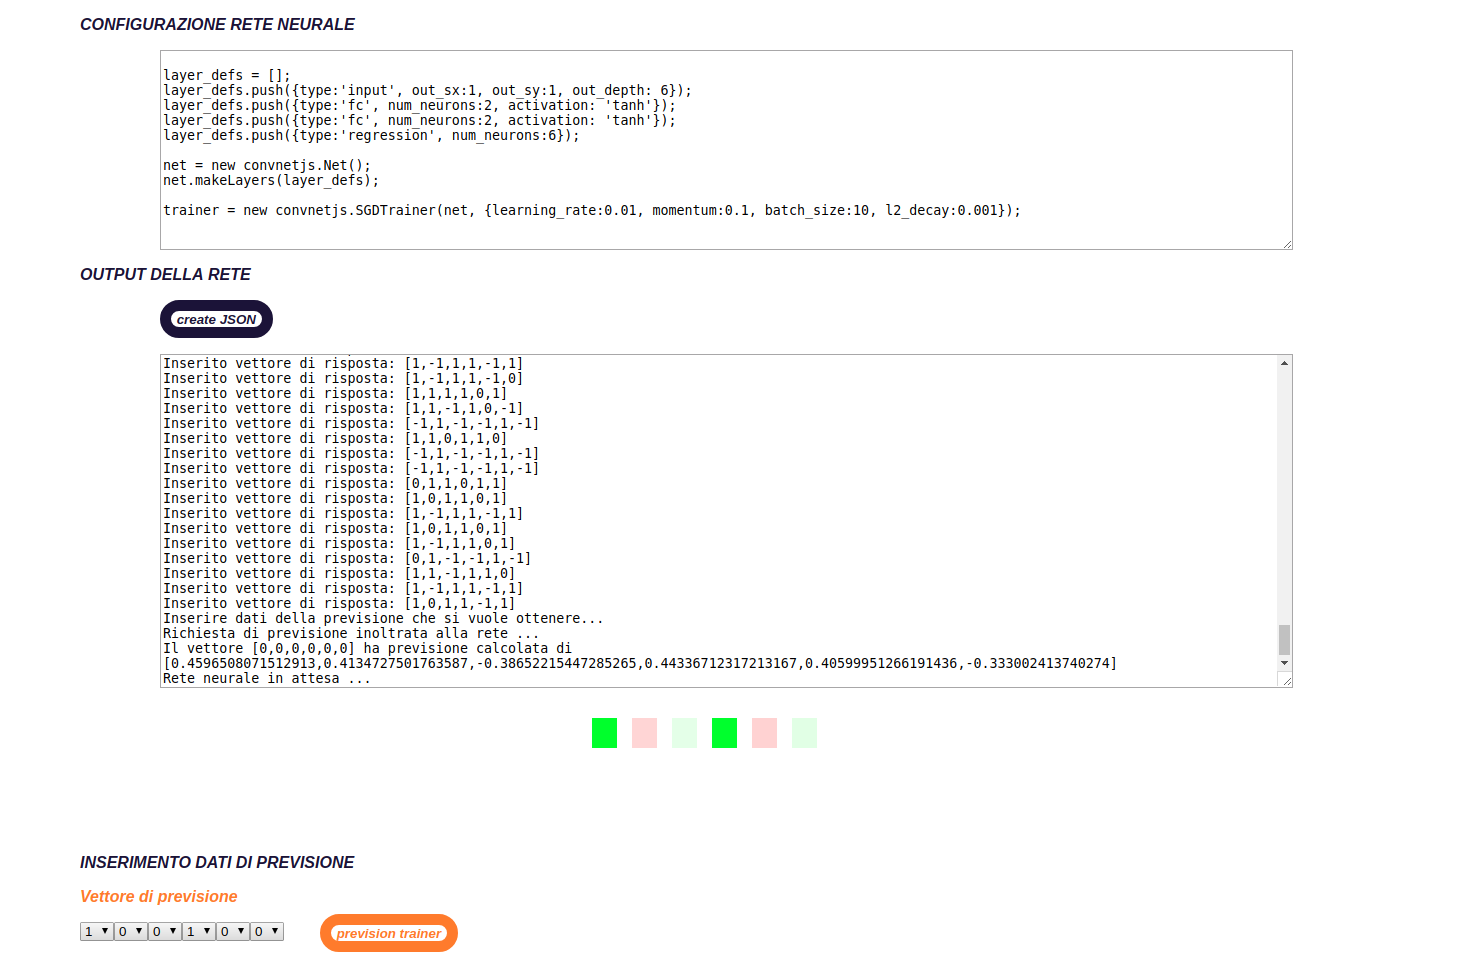
\includegraphics[width=0.90\linewidth]{./image/rete_prova-canvas.png}
	\caption{Rete di prova dopo lo sviluppo del canvas per le previsioni.}
	\label{Rete di prova dopo lo sviluppo del canvas per le previsioni.}
\end{figure}

\begin{figure}[H]
\centering
	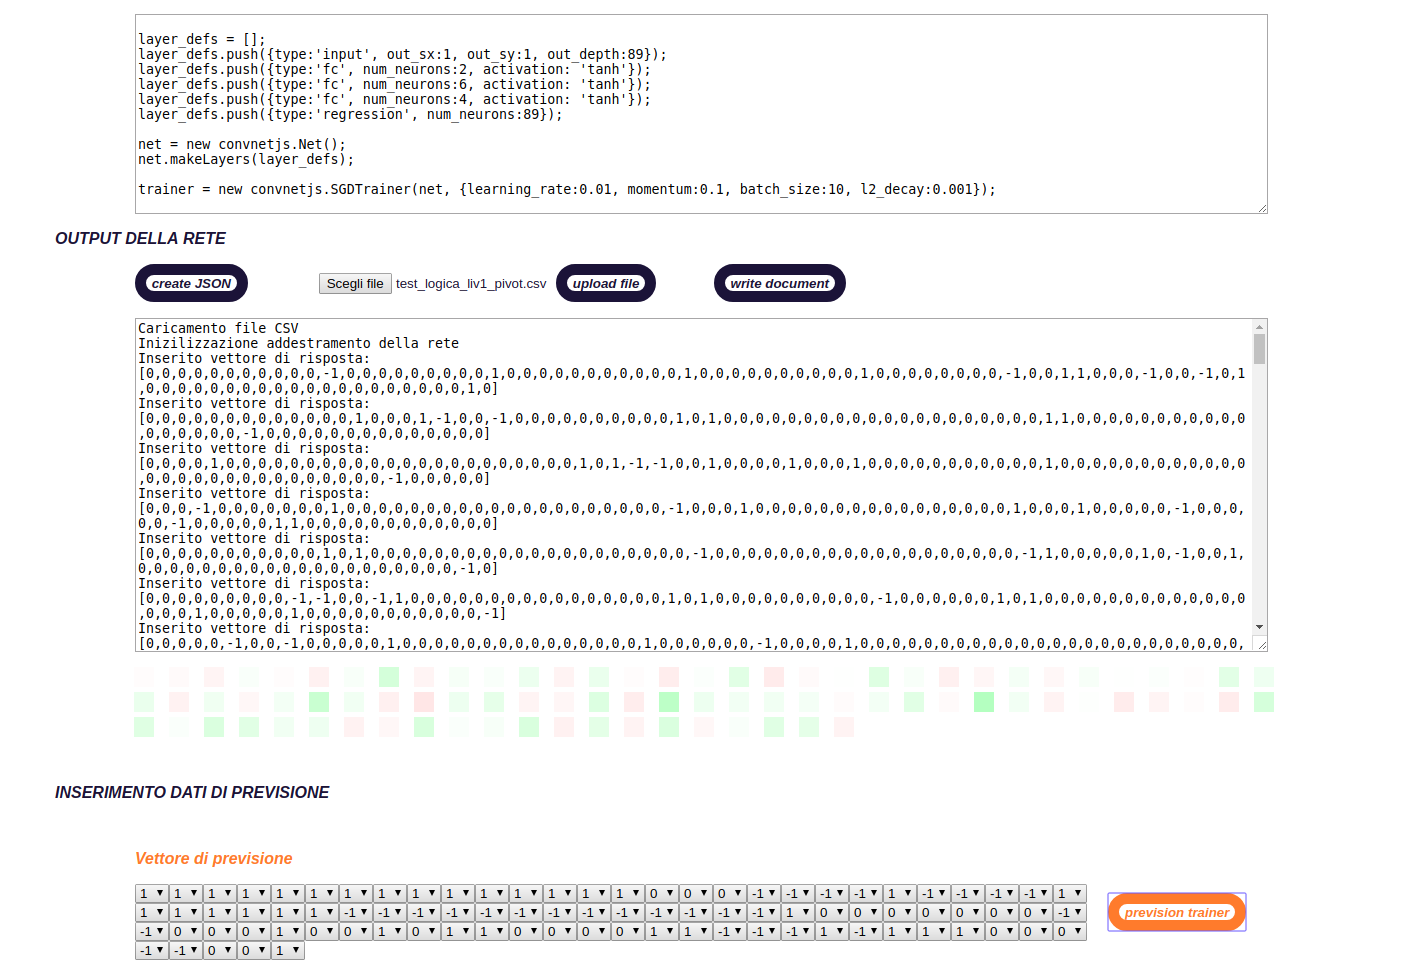
\includegraphics[width=0.90\linewidth]{./image/rete_db.png}
	\caption{Rete neurale del database aziendale.}
	\label{Rete neurale del database aziendale.}
\end{figure}
\noindent
Una prima architettura su cui ho deciso di analizzare i risultati della rete, basandomi anche sul quanto appreso dalla rete neurale di prova e dal numero di vettori di test utilizzati (1245 vettori x 89), \`e stata la seguente:
\begin{verbatim}
layer_defs = [];
layer_defs.push({type:'input', out_sx:1, out_sy:1, out_depth:89});
layer_defs.push({type:'fc', num_neurons:2, activation: 'tanh'});
layer_defs.push({type:'fc', num_neurons:6, activation: 'tanh'});
layer_defs.push({type:'fc', num_neurons:4, activation: 'tanh'});
layer_defs.push({type:'regression', num_neurons:89});

net = new convnetjs.Net();
net.makeLayers(layer_defs);

trainer = new convnetjs.SGDTrainer(net, {learning_rate:0.01,
momentum:0.1, batch_size:10, l2_decay:0.001});
\end{verbatim}
Ho aggiunto un layer e messo un numero di neuroni per layer in modo da formare un romboide. Devo verificare la bont\`a di questa mia scelta o se invece mi porta ad una situazione di overfitting.

\subsubsection{Natura delle domande contenute nel database aziendale}
\label{Natura delle domande contenute nel database aziendale}

Analizzando il training set dei vettori ho riscontrato tali correlazioni:
\begin{itemize}
\item Solo una piccola parte delle domande presenti nel database vengono svolte durante un colloquio con un candidato. In media una decina su 89 possibili.
\item Dalla rete sembra che le domande abbiano qualche correlazione, tuttavia la configurazione attuale ne rende difficoltosa l'individuazione. Quello che mi sembra opportuno ricercare testando l'architettura di della rete \`e che si vadano a formare dei cluster.
\end{itemize}


\subsubsection{Test e Documentazione}
\label{Test e Documentazione}
Durante la settimana dal 10/06 al 18/06 ho effettuato quanto definito al interno del Piano di Lavoro come "Test e Documentazione".

\paragraph{Test nella Rete di prova}\mbox{}\\\\
\label{Test nella Rete di prova}
\noindent
Architettura della rete utilizzata:\\
\begin{verbatim}layer_defs = [];
layer_defs.push({type:'input', out_sx:1, out_sy:1, out_depth:6});
layer_defs.push({type:'fc', num_neurons:2, activation: 'tanh'});
layer_defs.push({type:'fc', num_neurons:2, activation: 'tanh'});
layer_defs.push({type:'regression', num_neurons:6});

net = new convnetjs.Net();
net.makeLayers(layer_defs);

trainer = new convnetjs.SGDTrainer(net, {learning_rate:0.01,
 momentum:0.1, batch_size:10, l2_decay:0.001});
\end{verbatim}
\noindent



\begin{itemize}
\item \begin{verbatim}Il vettore [1,1,1,1,1,1] ha previsione calcolata di
[0.8521066399598267,0.898137375081856,0.9993098151218291,0.792190337086403,
0.811145866789799,0.9514731560722426]
\end{verbatim}

\begin{figure}[H]
\centering
	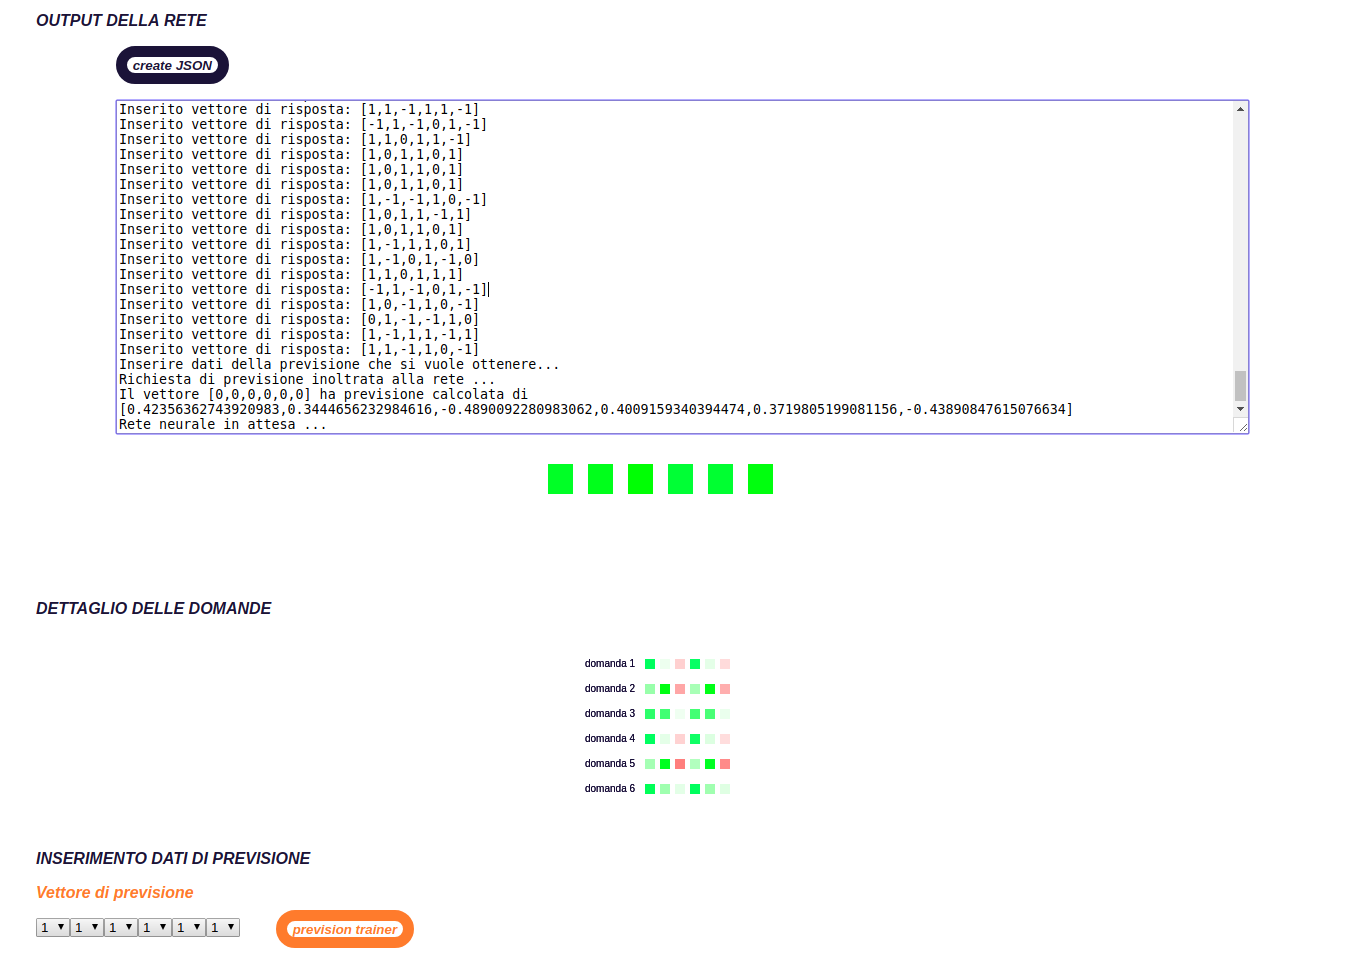
\includegraphics[width=0.90\linewidth]{./image/rete_prova-vp1.png}
	\caption{Risultato della rete di prova a seguito di un vettore di previsione [1, 1, 1, 1, 1, 1] in input.}
	\label{Risultato della rete di prova a seguito di un vettore di previsione [1, 1, 1, 1, 1, 1] in input.}
\end{figure}
Quanto mostrato dal dettaglio delle domande ha il seguente significato per un candidato:
\begin{itemize}
\item \textit{se la domanda 1 \`e settata a 1 (corretta)}: la rete prevede che la domanda 1 e 4 abbiano una probabilit\`a alta di essere risposte in modo corretto (verde); la 3 e 6 una probabilit\`a non eccessiva di venire risposte in modo sbagliato (rosa attenuato), la 2 e la 5 di non venire nemmeno poste (bianco con qualche minima sfumatura di verde).
\item \textit{se la domanda 2 \`e settata a 1 (corretta)}: la rete prevede che la domanda 1 e 4 abbiano una probabilit\`a non molto alta di essere risposte in modo corretto (bianco con qualche sfumatura di verde); la 3 e 6 una buona probabilit\`a di venire risposte in modo sbagliato (rosa), la 2 e la 5 di venire date in modo corretto (verde).
\item \textit{se la domanda 3 \`e settata a 1 (corretta)}: la rete prevede che la domanda 3 e 6 abbiano una probabilit\`a comunque bassa di essere risposte in modo corretto (bianco con qualche sfumatura di verde); la 1 e 4 con probabilit\`a di venire risposte in modo corretto (verde) perch\`e pi\`u semplici delle domande 3 e 6, la 2 e la 5 di venire risposte correttamente (verde).
\item \textit{se la domanda 4 \`e settata a 1 (corretta)}: la rete prevede un risultato  identico a quanto ottenuto dalla domanda 1.
\item \textit{se la domanda 5 \`e settata a 1 (corretta)}: la rete prevede un risultato similare a quanto ottenuto dalla domanda 2. Cambia solo quanto previsto dalle domande 3 e 6 che si presentano con un rosa un p\`o pi\`u intenso, in quanto con correlate alla coppia di domande 2 e 5.
\item \textit{se la domanda 6 \`e settata a 1 (corretta)}: la rete prevede un risultato simile a quanto ottenuto dalla domanda 3. La coppia 2 e 5 hanno una probabilit\`a minore di essere date correttamente (bianco con sfumature di verde) ma perch\`e non correlate alle domande 3 e 6.
\end{itemize}

\item \begin{verbatim}Il vettore [-1,-1,-1,-1,-1,-1] ha previsione calcolata di
[0.3440856175367477,-0.5026946644729329,-1.284368009920025,
0.35883842020377565,-0.37844446052773495,-1.1717763012412878]
\end{verbatim}

\begin{figure}[H]
\centering
	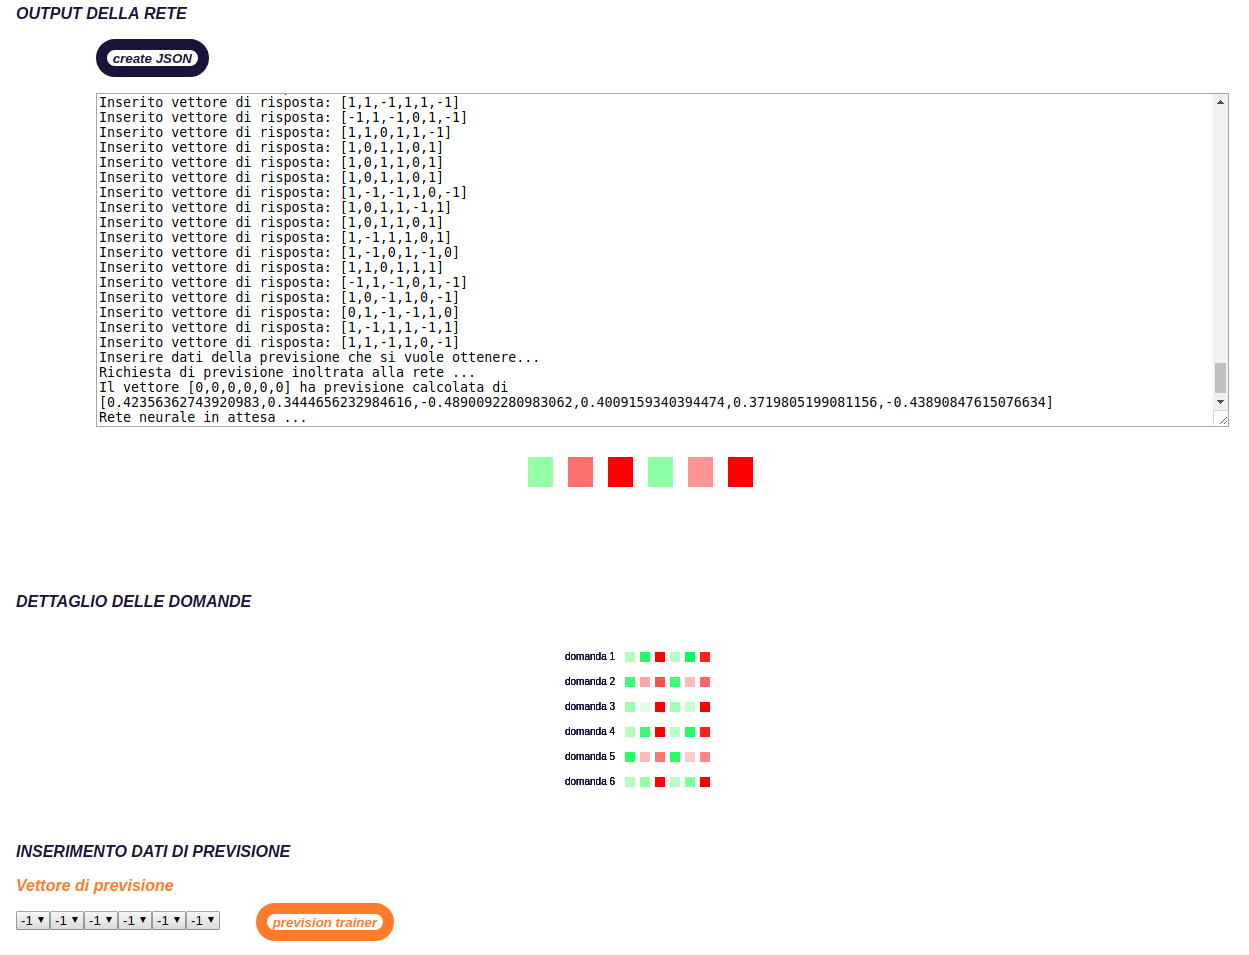
\includegraphics[width=0.90\linewidth]{./image/rete_prova-vpmeno1.png}
	\caption{Risultato della rete di prova a seguito di un vettore di previsione [-1, -1, -1, -1, -1, -1] in input.}
	\label{Risultato della rete di prova a seguito di un vettore di previsione [-1, -1, -1, -1, -1, -1] in input.}
\end{figure}
\begin{itemize}
\item \textit{se la domanda 1 \`e settata a -1 (non corretta)}: la rete prevede che la domanda 1 e 4 non abbiano una probabilit\`a alta di essere risposte in modo corretto (bianco con sfumature di verde); la 3 e 6 una probabilit\`a molto alta di venire risposte in modo sbagliato (rosso), la 2 e la 5 di non venire nemmeno poste (verde con qualche sfumatura di bianco).
\item \textit{se la domanda 2 \`e settata a -1 (non corretta)}: la rete prevede che la domanda 1 e 4 abbiano una probabilit\`a non molto alta di essere risposte in modo non corretto (verde con qualche sfumatura di bianco); la 3 e 6 una buona probabilit\`a di venire risposte in modo sbagliato (rosa), la 2 e la 5 di venire date in modo non corretto (rosa molto atenuato).
\item \textit{se la domanda 3 \`e settata a -1 (non corretta)}: la rete prevede che la domanda 3 e 6 abbiano una probabilit\`a comunque alta di essere risposte in modo non corretto (rosso); la 1 e 4 con bassa probabilit\`a di venire risposte in modo corretto (bianco con qualche sfumatura di verde) perch\`e pi\`u semplici delle domande 3 e 6, la 2 e la 5 di non venire nemmeno poste o comunque basso di venire risposto correttamente(bianco con sfumature di verde).
\item \textit{se la domanda 4 \`e settata a -1 (non corretta)}: la rete prevede un risultato  identico a quanto ottenuto dalla domanda 1.
\item \textit{se la domanda 5 \`e settata a -1 (non corretta)}: la rete prevede un risultato similare a quanto ottenuto dalla domanda 2. Cambia solo quanto previsto dalle domande 3 e 6 che si presentano con un rosa un p\`o meno intenso, in quanto non  correlate alla coppia di domande 2 e 5.
\item \textit{se la domanda 6 \`e settata a -1 (non corretta)}: la rete prevede un risultato simile a quanto ottenuto dalla domanda 3. La coppia 2 e 5 hanno una probabilit\`a maggiore di essere date correttamente (bianco con sfumature di verde) ma perch\`e non correlate alle domande 3 e 6.
\end{itemize}
\end{itemize}

\paragraph{Test nella Rete del database}\mbox{}\\
\label{Test nella Rete del database}
\noindent
\subparagraph{Architetture testate}\mbox{}\\\\
\label{Architetture testate}
\noindent
Durante tutto il periodo ho effettuato una serie di test su molteplici architettura della rete, con gradi di correlazione tra le domande pari al 100\% o con uno differenza massima di 5 punti colore rispetto al canvas risultante per ogni domanda.\\
Tuttavia non sono, durante questo periodo, riuscita ad individuare un'architettura sufficientemente stabile per prevedere risultati attendibili; a causa della molteplicit\`a di dati che hanno aumentato esponenzialmente  la complessit\`a di analisi rispetto alla Rete di prova. Tale complessit\`a \`e rimasta costante anche successivamente allo studio del contenuto delle domande nel database aziendale.
Architettura della rete utilizzata:
\begin{itemize}
\item \begin{verbatim}
layer_defs = [];
layer_defs.push({type:'input', out_sx:1, out_sy:1, out_depth:89});
layer_defs.push({type:'fc', num_neurons:2, activation: 'tanh'});
layer_defs.push({type:'fc', num_neurons:6, activation: 'tanh'});
layer_defs.push({type:'fc', num_neurons:4, activation: 'tanh'});
layer_defs.push({type:'regression', num_neurons:89});

net = new convnetjs.Net();
net.makeLayers(layer_defs);

trainer = new convnetjs.SGDTrainer(net, {learning_rate:0.01,
momentum:0.1, batch_size:10, l2_decay:0.001});
\end{verbatim}

\begin{figure}[H]
\centering
	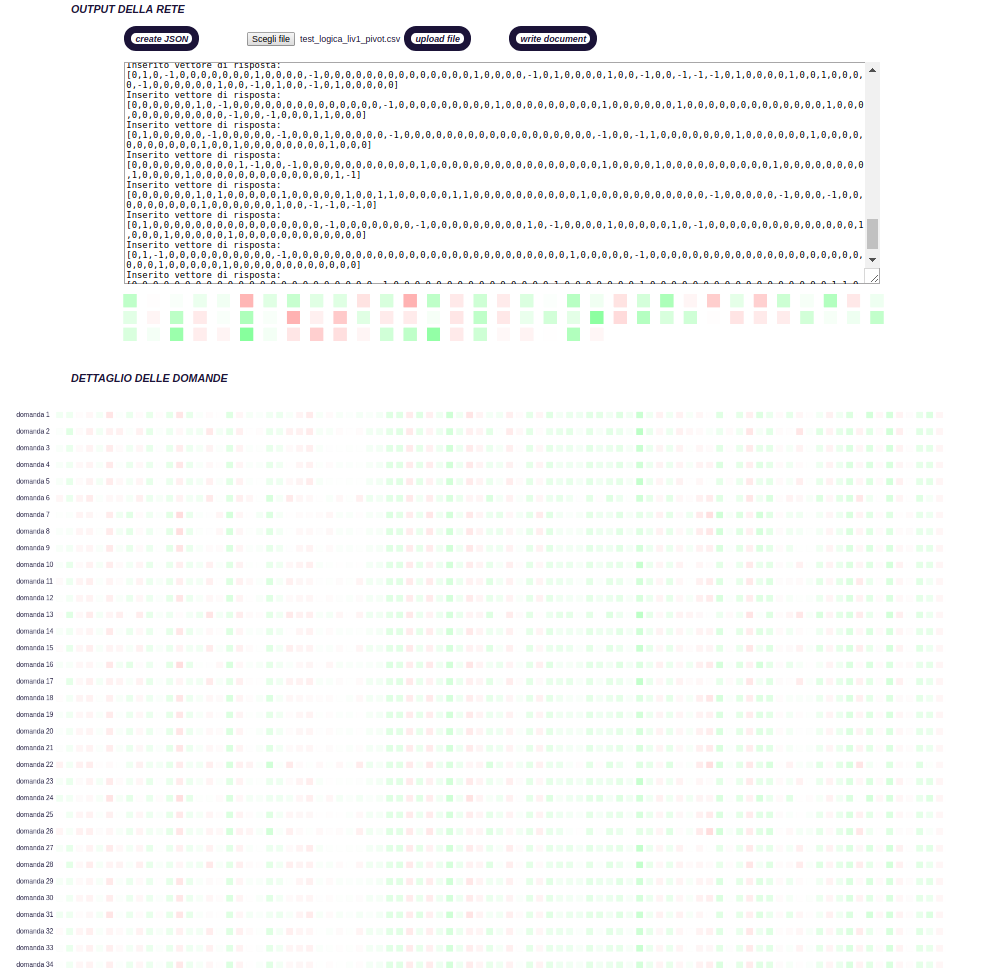
\includegraphics[width=0.90\linewidth]{./image/rete_db-vp1.png}
	\caption{Risultato della rete del database a seguito di un vettore di previsione [1, 1, 1, 1, 1, 1] in input.}
	\label{Risultato della rete del database a seguito di un vettore di previsione [1, 1, 1, 1, 1, 1] in input.}
\end{figure}

\begin{figure}[H]
\centering
	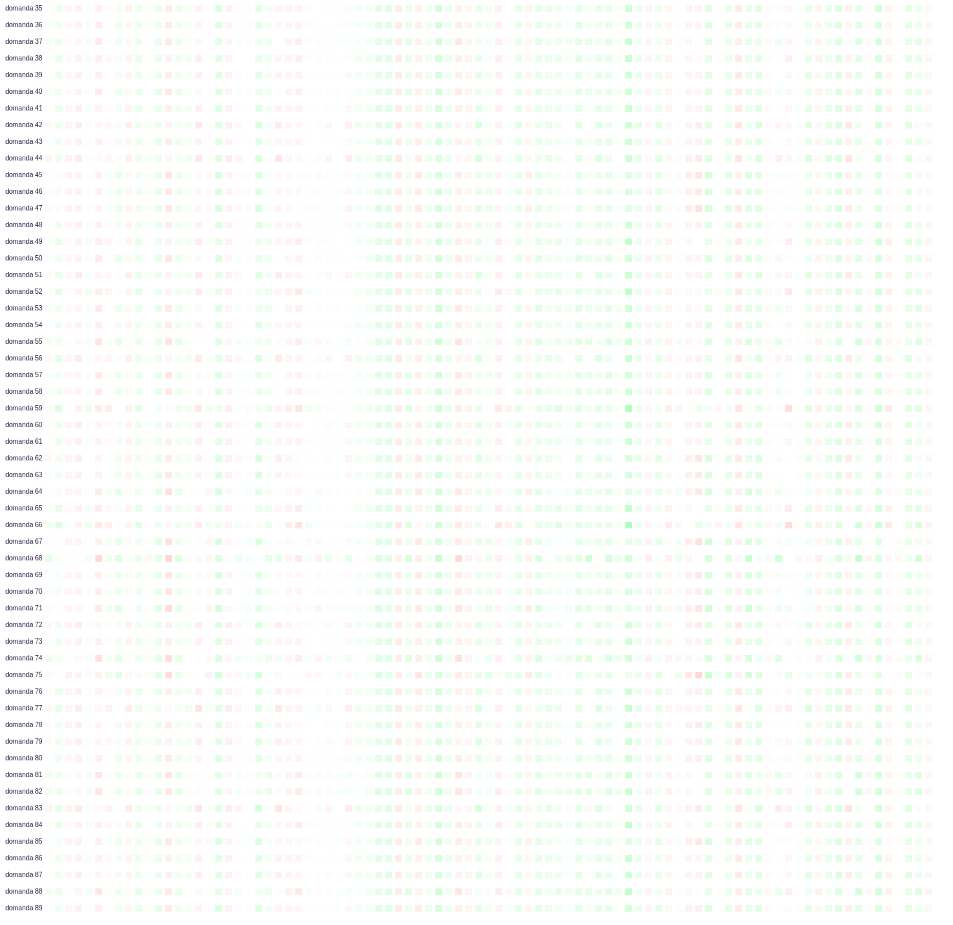
\includegraphics[width=0.90\linewidth]{./image/rete_db-vp1_2.png}
	\caption{Risultato della rete del database a seguito di un vettore di previsione [1, 1, 1, 1, 1, 1] in input.}
	\label{Risultato della rete del database a seguito di un vettore di previsione [1, 1, 1, 1, 1, 1] in input.}
\end{figure}
\noindent
Dagli screen della rete riportati sopra appare come "sembrano" domande:
\begin{enumerate}
\item Analisi verticale:
\begin{itemize}
\item \textit{semplici} la 18, 22, 34, 35, 37, 39, 41, 44, 48, 50, 51, 52, 53, 54, 55, 56, 57, 59, 60, 67, 69,  71, 72, 77, 79, 80, 82, 84, 87 e 88. Inoltre di queste sembrano in relazione ancora pi\`u stretta le domande 18, 22, 40 e 59.
\item \textit{difficili} la 3, 4, 6, 13, 16, 19, 24, 25, 26, 36, 38, 42, 43, 46, 49, 61, 63, 65, 66, 70, 78, 81, 85 e 89. Inoltre di queste sembrano in relazione ancora pi\`u stretta le domande 6, 13, 19, 36, 38, 42, 46 e 70.
\end{itemize}
\item Analisi orizzontale:
Appaiono in relazione stretta le seguenti domande:
\begin{itemize}
\item 2, 3, 4, 5;
\item 7, 8, 9;
\item 14, 16;
\item 20, 21;
\item 26, 32;
\item 29, 32
\item 33, 34, 35, 36, 38;
\item 39, 41, 43;
\item 46, 48;
\item 49, 52;
\item 50, 53;
\item 72, 79;
\item 81, 82;
\item 86, 87, 88.
\end{itemize}
\end{enumerate}

\begin{figure}[H]
\centering
	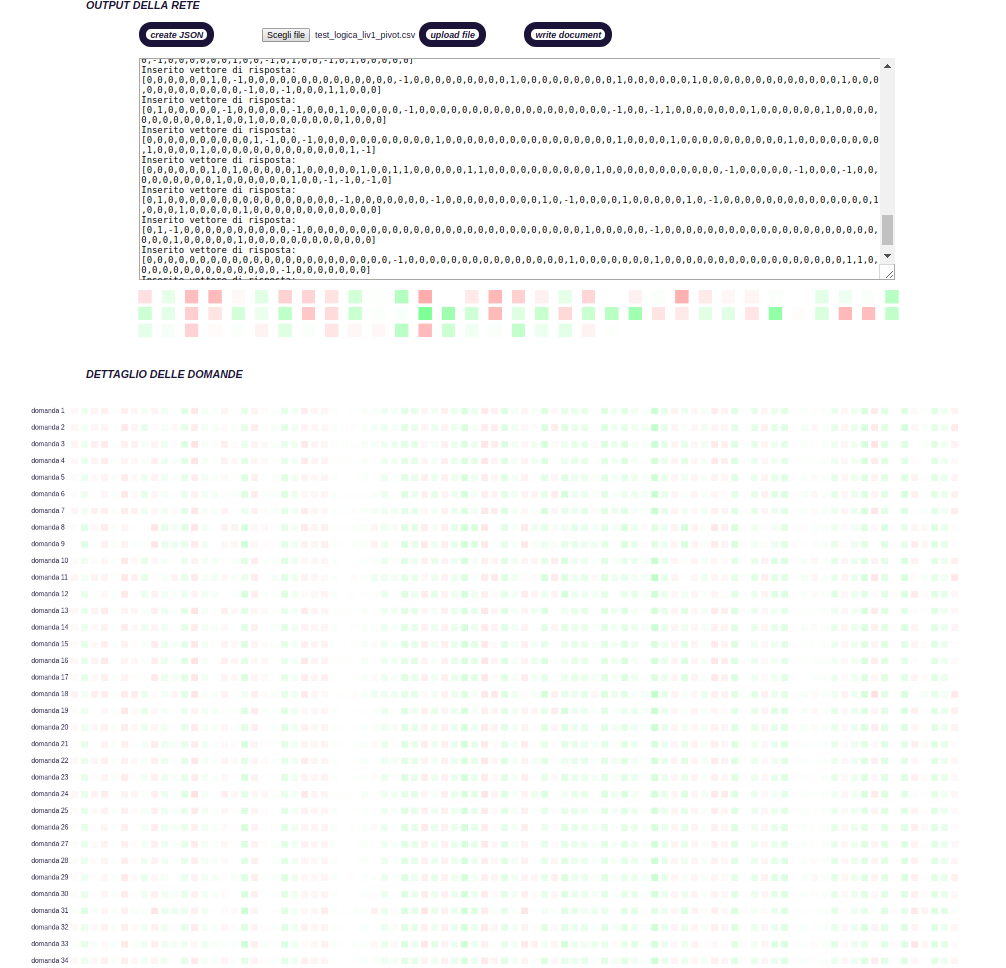
\includegraphics[width=0.90\linewidth]{./image/rete_db-vpmeno1.png}
	\caption{Risultato della rete del database a seguito di un vettore di previsione [-1, -1, -1, -1, -1, -1] in input.}
		\label{Risultato della rete del database a seguito di un vettore di previsione [-1, -1, -1, -1, -1, -1] in input.}
\end{figure}

\begin{figure}[H]
\centering
	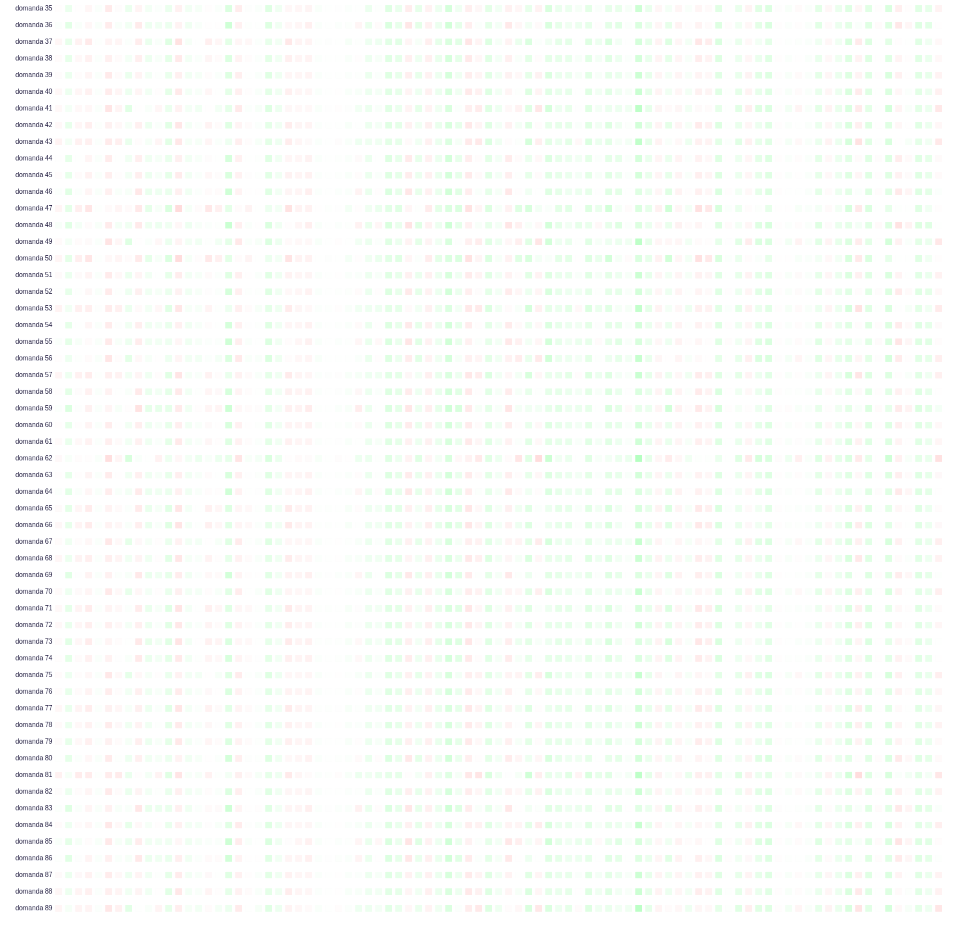
\includegraphics[width=0.90\linewidth]{./image/rete_db-vpmeno1_2.png}
	\caption{Risultato della rete del database a seguito di un vettore di previsione [-1, -1, -1, -1, -1, -1] in input.}
	\label{Risultato della rete del database a seguito di un vettore di previsione [-1, -1, -1, -1, -1, -1] in input.}
\end{figure}
\noindent
Dagli screen della rete riportati sopra appare come "sembrano" domande:
\begin{enumerate}
\item Analisi verticale:
\begin{itemize}
\item \textit{semplici} la 18, 22, 34, 35, 37, 38, 39, 41, 44, 48, 50, 51, 52, 54, 55, 56, 67, 69,  71, 72, 77, 79, 80, 82, 84, 87 e 88. Inoltre di queste sembrano in relazione ancora pi\`u stretta le domande 18, 22, 38, 52 e 57.
\item \textit{difficili} la 3, 4, 6, 13, 19, 27, 36, 38, 42, 43, 46, 61, 62, 65, 70. Inoltre di queste sembrano in relazione ancora pi\`u stretta le domande 6, 13, 19, 36, 38, 42, 46, 61 e 62.
\end{itemize}
\item Analisi orizzontale:
Appaiono in relazione stretta le seguenti domande:
\begin{itemize}
\item rimaste consistenti con il vettore [1, 1, 1, 1, 1, 1].
\end{itemize}
\end{enumerate}


\item \begin{verbatim}
layer_defs = [];
layer_defs.push({type:'input', out_sx:1, out_sy:1, out_depth:89});
layer_defs.push({type:'fc', num_neurons:12, activation: 'tanh'});
layer_defs.push({type:'regression', num_neurons:89});

net = new convnetjs.Net();
net.makeLayers(layer_defs);

trainer = new convnetjs.SGDTrainer(net, {learning_rate:0.01, momentum:0.1
, batch_size:10, l2_decay:0.001});
\end{verbatim}
Noto che aumentando il numero di neuroni sull'unico layer esistente, il valore della domanda corrispondente al vettore della previsione sembra sempre pi\`u marcato, segno che la rete "impara troppo" e ricade nel restituire l'immagine stessa del vettore previsione.

\begin{figure}[H]
\centering
	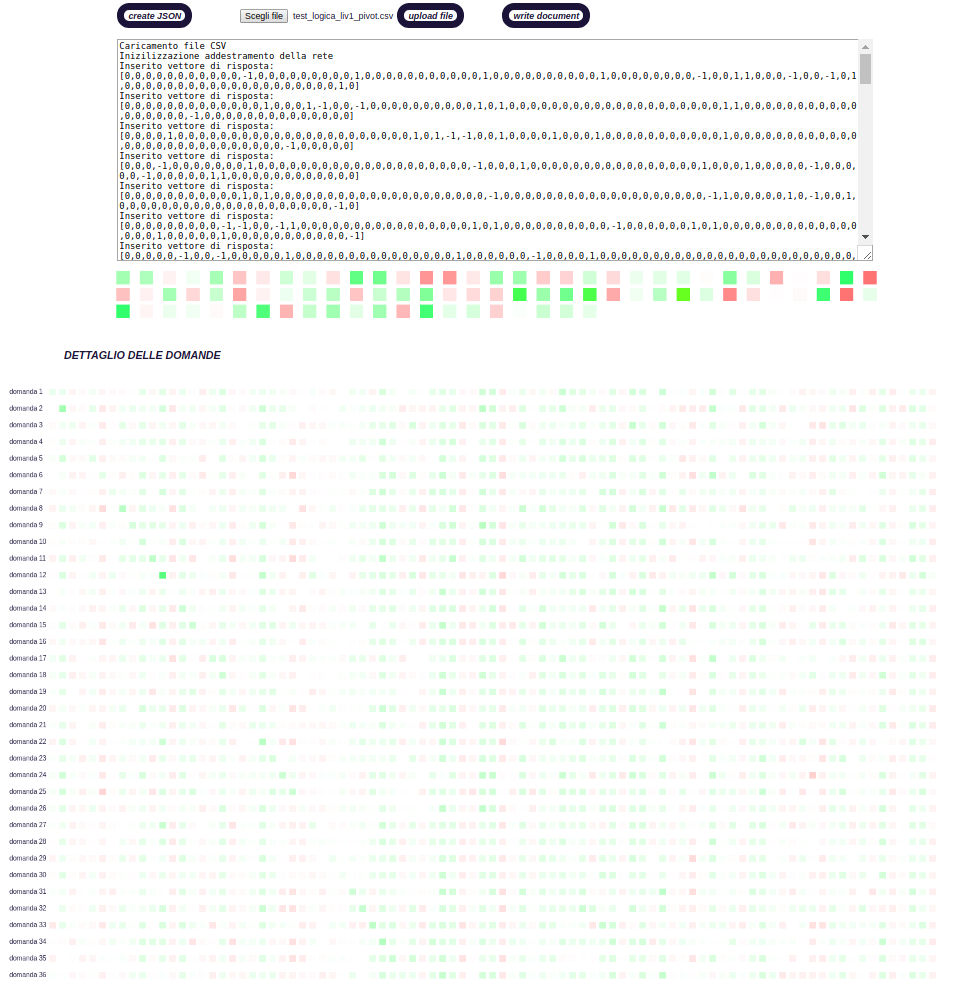
\includegraphics[width=0.90\linewidth]{./image/rete_db-vp1architettura2.png}
	\caption{Risultato della rete del database a seguito di un vettore di previsione [1, 1, 1, 1, 1, 1] in input.}
	\label{Risultato della rete del database a seguito di un vettore di previsione [1, 1, 1, 1, 1, 1] in input.}
\end{figure}

\begin{figure}[H]
\centering
	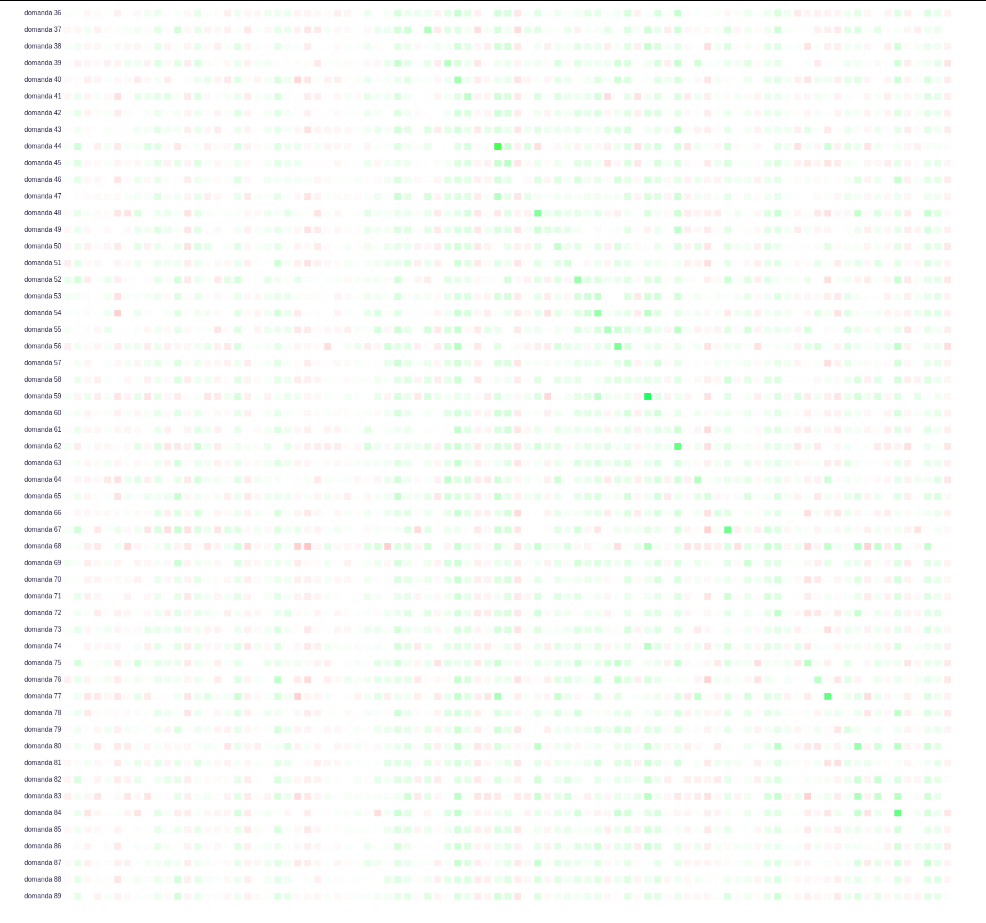
\includegraphics[width=0.90\linewidth]{./image/rete_db-vp1_2architettura2.png}
	\caption{Risultato della rete del database a seguito di un vettore di previsione [1, 1, 1, 1, 1, 1] in input.}
	\label{Risultato della rete del database a seguito di un vettore di previsione [1, 1, 1, 1, 1, 1] in input.}
\end{figure}


Dagli screen della rete riportati sopra appare come la situazione appare meno lineare del caso analizzato precedentemente. 
Le domande non vengono separate per linee rete; ma per aree di relazione.


Dagli screen della rete riportati sopra appare come "sembrano" domande:
\begin{enumerate}
\item Analisi verticale:
\begin{itemize}
\item \textit{semplici} la 18, 22, 34, 35, 37, 39, 41, 44, 48, 50, 51, 52, 53, 54, 55, 56, 57, 59, 60, 67, 69,  71, 72, 77, 79, 80, 82, 84, 87 e 88. Inoltre di queste sembrano in relazione ancora pi\`u stretta le domande 18, 22, 40 e 59.
\item \textit{difficili} la 3, 4, 6, 13, 16, 19, 24, 25, 26, 36, 38, 42, 43, 46, 49, 61, 63, 65, 66, 70, 78, 81, 85 e 89. Inoltre di queste sembrano in relazione ancora pi\`u stretta le domande 6, 13, 19, 36, 38, 42, 46 e 70.
\end{itemize}
\item Analisi orizzontale:
Appaiono in relazione stretta le seguenti domande:
\begin{itemize}
\item Vengono meno le relazioni individuate precedentemente.
\end{itemize}
\end{enumerate}
\noindent


\item \begin{verbatim}
layer_defs = [];
layer_defs.push({type:'input', out_sx:1, out_sy:1, out_depth:89});
layer_defs.push({type:'fc', num_neurons:2, activation: 'tanh'});
layer_defs.push({type:'fc', num_neurons:6, activation: 'tanh'});
layer_defs.push({type:'fc', num_neurons:4, activation: 'tanh'});
layer_defs.push({type:'regression', num_neurons:89});

net = new convnetjs.Net();
net.makeLayers(layer_defs);

trainer = new convnetjs.SGDTrainer(net, {learning_rate:0.01,
momentum:0.1, batch_size:10, l2_decay:0.001});
\end{verbatim}

\item \begin{verbatim}
layer_defs = [];
layer_defs.push({type:'input', out_sx:1, out_sy:1, out_depth:89});
layer_defs.push({type:'fc', num_neurons:12, activation: 'tanh'});
layer_defs.push({type:'regression', num_neurons:89});

net = new convnetjs.Net();
net.makeLayers(layer_defs);

trainer = new convnetjs.SGDTrainer(net, {learning_rate:0.01,
momentum:0.1, batch_size:10, l2_decay:0.001});
\end{verbatim}

\item \begin{verbatim}
layer_defs = [];
layer_defs.push({type:'input', out_sx:1, out_sy:1, out_depth:89});
layer_defs.push({type:'fc', num_neurons:12, activation: 'tanh'});
layer_defs.push({type:'fc', num_neurons:8, activation: 'tanh'});
layer_defs.push({type:'fc', num_neurons:6, activation: 'tanh'});
layer_defs.push({type:'fc', num_neurons:4, activation: 'tanh'});
layer_defs.push({type:'regression', num_neurons:89});

net = new convnetjs.Net();
net.makeLayers(layer_defs);

trainer = new convnetjs.SGDTrainer(net, {learning_rate:0.01, 
momentum:0.1, batch_size:10, l2_decay:0.001});
\end{verbatim}



\item \begin{verbatim}
layer_defs = [];
layer_defs.push({type:'input', out_sx:1, out_sy:1, out_depth:89});
layer_defs.push({type:'fc', num_neurons:2, activation: 'tanh'});
layer_defs.push({type:'fc', num_neurons:6, activation: 'tanh'});
layer_defs.push({type:'fc', num_neurons:6, activation: 'tanh'});
layer_defs.push({type:'fc', num_neurons:4, activation: 'tanh'});
layer_defs.push({type:'regression', num_neurons:89});

net = new convnetjs.Net();
net.makeLayers(layer_defs);

trainer = new convnetjs.SGDTrainer(net, {learning_rate:0.01, 
momentum:0.1, batch_size:10, l2_decay:0.001})
\end{verbatim}



\item \begin{verbatim}
layer_defs = [];
layer_defs.push
({type:'input', out_sx:1, out_sy:1, out_depth:89});
layer_defs.push({type:'fc', num_neurons:2, activation: 'tanh'});
layer_defs.push({type:'fc', num_neurons:4, activation: 'tanh'});
layer_defs.push({type:'fc', num_neurons:6, activation: 'tanh'});
layer_defs.push({type:'fc', num_neurons:4, activation: 'tanh'});
layer_defs.push({type:'regression', num_neurons:89});

net = new convnetjs.Net();
net.makeLayers(layer_defs);

trainer = new convnetjs.SGDTrainer(net, {learning_rate:0.01, 
momentum:0.1, batch_size:10, l2_decay:0.001});
\end{verbatim}


\item \begin{verbatim}
layer_defs = [];
layer_defs.push({type:'input', out_sx:1, out_sy:1, out_depth:89});
layer_defs.push({type:'fc', num_neurons:2, activation: 'tanh'});
layer_defs.push({type:'fc', num_neurons:6, activation: 'tanh'});
layer_defs.push({type:'fc', num_neurons:2, activation: 'tanh'});
layer_defs.push({type:'regression', num_neurons:89});

net = new convnetjs.Net();
net.makeLayers(layer_defs);

trainer = new convnetjs.SGDTrainer(net, {learning_rate:0.01, 
momentum:0.1, batch_size:10, l2_decay:0.001});
\end{verbatim}


\item \begin{verbatim}
layer_defs = [];
layer_defs.push({type:'input', out_sx:1, out_sy:1, out_depth:89});
layer_defs.push({type:'fc', num_neurons:2, activation: 'tanh'});
layer_defs.push({type:'fc', num_neurons:4, activation: 'tanh'});
layer_defs.push({type:'fc', num_neurons:2, activation: 'tanh'});
layer_defs.push({type:'regression', num_neurons:89});

net = new convnetjs.Net();
net.makeLayers(layer_defs);

trainer = new convnetjs.SGDTrainer(net, {learning_rate:0.01, 
momentum:0.1, batch_size:10, l2_decay:0.001});
\end{verbatim}


\item \begin{verbatim}
layer_defs = [];
layer_defs.push({type:'input', out_sx:1, out_sy:1, out_depth:89});
layer_defs.push({type:'fc', num_neurons:2, activation: 'tanh'});
layer_defs.push({type:'fc', num_neurons:2, activation: 'tanh'});
layer_defs.push({type:'regression', num_neurons:89});

net = new convnetjs.Net();
net.makeLayers(layer_defs);

trainer = new convnetjs.SGDTrainer(net, {learning_rate:0.01, 
momentum:0.1, batch_size:10, l2_decay:0.001});
\end{verbatim}

\item \begin{verbatim}
layer_defs = [];
layer_defs.push({type:'input', out_sx:1, out_sy:1, out_depth:89});
layer_defs.push({type:'fc', num_neurons:4, activation: 'tanh'});
layer_defs.push({type:'fc', num_neurons:4, activation: 'tanh'});
layer_defs.push({type:'regression', num_neurons:89});

net = new convnetjs.Net();
net.makeLayers(layer_defs);

trainer = new convnetjs.SGDTrainer(net, {learning_rate:0.01, 
momentum:0.1, batch_size:10, l2_decay:0.001});
\end{verbatim}


\item \begin{verbatim}
layer_defs = [];
layer_defs.push({type:'input', out_sx:1, out_sy:1, out_depth:89});
layer_defs.push({type:'fc', num_neurons:3, activation: 'tanh'});
layer_defs.push({type:'fc', num_neurons:3, activation: 'tanh'});
layer_defs.push({type:'regression', num_neurons:89});

net = new convnetjs.Net();
net.makeLayers(layer_defs);

trainer = new convnetjs.SGDTrainer(net, {learning_rate:0.01,
 momentum:0.1, batch_size:10, l2_decay:0.001});
\end{verbatim}


\item \begin{verbatim}
layer_defs = [];
layer_defs.push({type:'input', out_sx:1, out_sy:1, out_depth:89});
layer_defs.push({type:'fc', num_neurons:3, activation: 'tanh'});
layer_defs.push({type:'fc', num_neurons:2, activation: 'tanh'});
layer_defs.push({type:'regression', num_neurons:89});

net = new convnetjs.Net();
net.makeLayers(layer_defs);

trainer = new convnetjs.SGDTrainer(net, {learning_rate:0.01, 
momentum:0.1, batch_size:10, l2_decay:0.001});
\end{verbatim}


\item \begin{verbatim}
layer_defs = [];
layer_defs.push({type:'input', out_sx:1, out_sy:1, out_depth:89});
layer_defs.push({type:'fc', num_neurons:2, activation: 'tanh'});
layer_defs.push({type:'fc', num_neurons:3, activation: 'tanh'});
layer_defs.push({type:'fc', num_neurons:1, activation: 'tanh'});
layer_defs.push({type:'regression', num_neurons:89});

net = new convnetjs.Net();
net.makeLayers(layer_defs);

trainer = new convnetjs.SGDTrainer(net, {learning_rate:0.01, 
momentum:0.1, batch_size:10, l2_decay:0.001});
\end{verbatim}


\item \begin{verbatim}
layer_defs = [];
layer_defs.push({type:'input', out_sx:1, out_sy:1, out_depth:89});
layer_defs.push({type:'fc', num_neurons:2, activation: 'tanh'});
layer_defs.push({type:'fc', num_neurons:3, activation: 'tanh'});
layer_defs.push({type:'fc', num_neurons:2, activation: 'tanh'});
layer_defs.push({type:'regression', num_neurons:89});

net = new convnetjs.Net();
net.makeLayers(layer_defs);

trainer = new convnetjs.SGDTrainer(net, {learning_rate:0.01, 
momentum:0.1, batch_size:10, l2_decay:0.001});
\end{verbatim}


\item \begin{verbatim}
layer_defs = [];
layer_defs.push({type:'input', out_sx:1, out_sy:1, out_depth:89});
layer_defs.push({type:'fc', num_neurons:2, activation: 'tanh'});
layer_defs.push({type:'fc', num_neurons:4, activation: 'tanh'});
layer_defs.push({type:'fc', num_neurons:1, activation: 'tanh'});
layer_defs.push({type:'regression', num_neurons:89});

net = new convnetjs.Net();
net.makeLayers(layer_defs);

trainer = new convnetjs.SGDTrainer(net, {learning_rate:0.01, 
momentum:0.1, batch_size:10, l2_decay:0.001});
\end{verbatim}

\item \begin{verbatim}
layer_defs = [];
layer_defs.push({type:'input', out_sx:1, out_sy:1, out_depth:89});
layer_defs.push({type:'fc', num_neurons:2, activation: 'tanh'});
layer_defs.push({type:'fc', num_neurons:5, activation: 'tanh'});
layer_defs.push({type:'fc', num_neurons:1, activation: 'tanh'});
layer_defs.push({type:'regression', num_neurons:89});

net = new convnetjs.Net();
net.makeLayers(layer_defs);

trainer = new convnetjs.SGDTrainer(net, {learning_rate:0.01,
momentum:0.1, batch_size:10, l2_decay:0.001});
\end{verbatim}


\item \begin{verbatim}
layer_defs = [];
layer_defs.push({type:'input', out_sx:1, out_sy:1, out_depth:89});
layer_defs.push({type:'fc', num_neurons:1, activation: 'tanh'});
layer_defs.push({type:'fc', num_neurons:4, activation: 'tanh'});
layer_defs.push({type:'fc', num_neurons:1, activation: 'tanh'});
layer_defs.push({type:'regression', num_neurons:89});

net = new convnetjs.Net();
net.makeLayers(layer_defs);

trainer = new convnetjs.SGDTrainer(net, {learning_rate:0.01, 
momentum:0.1, batch_size:10, l2_decay:0.001});
\end{verbatim}

\item \begin{verbatim}
layer_defs = [];
layer_defs.push({type:'input', out_sx:1, out_sy:1, out_depth:89});
layer_defs.push({type:'fc', num_neurons:3, activation: 'tanh'});
layer_defs.push({type:'fc', num_neurons:4, activation: 'tanh'});
layer_defs.push({type:'fc', num_neurons:1, activation: 'tanh'});
layer_defs.push({type:'regression', num_neurons:89});

net = new convnetjs.Net();
net.makeLayers(layer_defs);

trainer = new convnetjs.SGDTrainer(net, {learning_rate:0.01, 
momentum:0.1, batch_size:10, l2_decay:0.001});
\end{verbatim}


\item \begin{verbatim}
layer_defs = [];
layer_defs.push({type:'input', out_sx:1, out_sy:1, out_depth:89});
layer_defs.push({type:'fc', num_neurons:6, activation: 'tanh'});
layer_defs.push({type:'fc', num_neurons:6, activation: 'tanh'});
layer_defs.push({type:'fc', num_neurons:6, activation: 'tanh'});
layer_defs.push({type:'fc', num_neurons:6, activation: 'tanh'});
layer_defs.push({type:'regression', num_neurons:89});

net = new convnetjs.Net();
net.makeLayers(layer_defs);

trainer = new convnetjs.SGDTrainer(net, {learning_rate:0.01, 
momentum:0.1, batch_size:10, l2_decay:0.001});
\end{verbatim}

\item \begin{verbatim}
layer_defs = [];
layer_defs.push({type:'input', out_sx:1, out_sy:1, out_depth:89});
layer_defs.push({type:'fc', num_neurons:18, activation: 'tanh'});
layer_defs.push({type:'fc', num_neurons:18, activation: 'tanh'});
layer_defs.push({type:'regression', num_neurons:89});

net = new convnetjs.Net();
net.makeLayers(layer_defs);

trainer = new convnetjs.SGDTrainer(net, {learning_rate:0.01, 
momentum:0.1, batch_size:10, l2_decay:0.001});
\end{verbatim}

\item \begin{verbatim}
layer_defs = [];
layer_defs.push({type:'input', out_sx:1, out_sy:1, out_depth:89});
layer_defs.push({type:'fc', num_neurons:18, activation: 'tanh'});
layer_defs.push({type:'fc', num_neurons:18, activation: 'tanh'});
layer_defs.push({type:'fc', num_neurons:18, activation: 'tanh'});
layer_defs.push({type:'regression', num_neurons:89});

net = new convnetjs.Net();
net.makeLayers(layer_defs);

trainer = new convnetjs.SGDTrainer(net, {learning_rate:0.01, 
momentum:0.1, batch_size:10, l2_decay:0.001});
\end{verbatim}

\item \begin{verbatim}
layer_defs = [];
layer_defs.push({type:'input', out_sx:1, out_sy:1, out_depth:89});
layer_defs.push({type:'fc', num_neurons:2, activation: 'tanh'});
layer_defs.push({type:'fc', num_neurons:3, activation: 'tanh'});
layer_defs.push({type:'fc', num_neurons:2, activation: 'tanh'});
layer_defs.push({type:'fc', num_neurons:1, activation: 'tanh'});
layer_defs.push({type:'regression', num_neurons:89});

net = new convnetjs.Net();
net.makeLayers(layer_defs);

trainer = new convnetjs.SGDTrainer(net, {learning_rate:0.01,
 momentum:0.1, batch_size:10, l2_decay:0.001});
\end{verbatim}

\item \begin{verbatim}
layer_defs = [];
layer_defs.push({type:'input', out_sx:1, out_sy:1, out_depth:89});
layer_defs.push({type:'fc', num_neurons:2, activation: 'tanh'});
layer_defs.push({type:'fc', num_neurons:3, activation: 'tanh'});
layer_defs.push({type:'fc', num_neurons:3, activation: 'tanh'});
layer_defs.push({type:'fc', num_neurons:1, activation: 'tanh'});
layer_defs.push({type:'regression', num_neurons:89});

net = new convnetjs.Net();
net.makeLayers(layer_defs);

trainer = new convnetjs.SGDTrainer(net, {learning_rate:0.01, 
momentum:0.1, batch_size:10, l2_decay:0.001});
\end{verbatim}

\item \begin{verbatim}
layer_defs = [];
layer_defs.push({type:'input', out_sx:1, out_sy:1, out_depth:89});
layer_defs.push({type:'fc', num_neurons:2, activation: 'tanh'});
layer_defs.push({type:'fc', num_neurons:6, activation: 'tanh'});
layer_defs.push({type:'fc', num_neurons:3, activation: 'tanh'});
layer_defs.push({type:'fc', num_neurons:1, activation: 'tanh'});
layer_defs.push({type:'regression', num_neurons:89});

net = new convnetjs.Net();
net.makeLayers(layer_defs);

trainer = new convnetjs.SGDTrainer(net, {learning_rate:0.01, 
momentum:0.1, batch_size:10, l2_decay:0.001});
\end{verbatim}

\item \begin{verbatim}
layer_defs = [];
layer_defs.push({type:'input', out_sx:1, out_sy:1, out_depth:89});
layer_defs.push({type:'fc', num_neurons:2, activation: 'tanh'});
layer_defs.push({type:'fc', num_neurons:6, activation: 'tanh'});
layer_defs.push({type:'fc', num_neurons:4, activation: 'tanh'});
layer_defs.push({type:'fc', num_neurons:1, activation: 'tanh'});
layer_defs.push({type:'regression', num_neurons:89});

net = new convnetjs.Net();
net.makeLayers(layer_defs);

trainer = new convnetjs.SGDTrainer(net, {learning_rate:0.01, 
momentum:0.1, batch_size:10, l2_decay:0.001});
\end{verbatim}


\item \begin{verbatim}
layer_defs = [];
layer_defs.push({type:'input', out_sx:1, out_sy:1, out_depth:89});
layer_defs.push({type:'fc', num_neurons:8, activation: 'tanh'});
layer_defs.push({type:'fc', num_neurons:8, activation: 'tanh'});
layer_defs.push({type:'regression', num_neurons:89});

net = new convnetjs.Net();
net.makeLayers(layer_defs);

trainer = new convnetjs.SGDTrainer(net, {learning_rate:0.01, 
momentum:0.1, batch_size:10, l2_decay:0.001});
\end{verbatim}
\noindent
L'obiettivo dei miei test \`e stato individuare una configurazione abbastanza "forte" da permettere il riscontro di correlazioni e dei possibili cluster esistenti con il solo ausilio della Rete. Tuttavia per proseguire il mio studio \`e indispensabile che mi avvalga di anche altri strumenti di supporto. Il prossimo passo \`e costruire un modello di dati mediante la tecnica di {P}rincipal \textbf{C}omponent \textbf{A}nalysis .
\end{itemize}

\subsection{Funzionalit\`a offerte dall'interfaccia della Rete neurale delle domande nel databse}
\label{Funzionalita offerte dall'interfaccia della Rete neurale}
La Rete neurale sviluppata \`e stata pensata per una persona che deve svolgere analisi dei dati mirata alla previsione dei risultati su un caso studio specifico (la dimensione \`e fissata a 89). L'applicativo realizzato offre le seguenti funzionalit\`a:
\begin{itemize}
\item Caricamento dei dati con l'utilizzo di formati \textit{CSV} o \textit{TXT};
\item Possibilit\`a di visualizzare i dati caricati direttamente su pagina web. Ogni risposta viene presentata con codice di test e codice della domanda;
\item Possibilit\`a di visualizzare i dati caricati nella Rete mediante formato JSON. In questo modo la rete post apprendimento viene salvata ed \`e possibile visualizzare come ogni nodo pesa ogni variabile. Inoltre l'ultima rete salvata pu\`o venire caricata in ogni momento e riutilizzata;
\item La Rete neurale \`e fornita di due textarea: 
\begin{itemize}
\item La prima che permette la visualizzazione dell'architettura in uso, con indicazione della tipologia di trainer utilizzato. Questa sezione permette la modifica delle variabili di configurazione\footnote{Ogni modifica del numero di neuroni espressi nella regressione deve provocare la modifica del file di previsione della rete.};
\item La seconda che consente la visualizzazione dei risultati ottenuti dalla Rete.
\end{itemize}
\item \`E possibile settare la previsione che si vuole ottenere, mediante un'area di inserimento con box a radio. Il valore di default imposto \`e 0. 
\item Per ogni previsione svolta viene visualizzato non solo il risultato della stessa numericamente espresso all'interno della seconda textarea; ma viene anche rappresentato visivamente per mezzo di canvas;
\item \`E offerta la funzionalit\`a di inserimento dei parametri di differenziale con filtro sulla colorazione, che permette l'indicazione dei cluster esistenti;
\item \`E possibile visualizzare per ogni elemento soggetto alla previsione il dettaglio della previsione stessa. Questa viene presentata visivamente per mezzo di canvas;
\item \`E possibile eliminare lo storico dei dati stampati nella seconda textarea.
\end{itemize}


\subsubsection{Diagrammi dei casi d'uso}
\label{casi d'uso}
\paragraph{Attori}\mbox{}\\
\label{Attori}
Gli \textit{attori} esistenti all'interno del sistema che si occupano di interagire con esso sono:
\begin{itemize}
\item \textbf{Utente osservatore}: utente che agisce  direttamente sulla Rete neurale, in modo da effettuare osservazioni ed analisi dei dati di interesse.
\end{itemize}

\paragraph{Casi d'uso}\mbox{}\\
\label{Casi d'uso}
\noindent
\subparagraph{UC0\_g: Operazioni utente - Visione generale interfacciamento con la Rete neurale}\mbox{}\\\\
\label{UC0_g: Operazioni utente - Visione generale interfacciamento con la Rete neurale}
\textit{Per ogni funzionalit\`a espressa in UC0\_g \`e stato creato un diagramma differente in modo da evitare connessioni tra le frecce e una corretta visualizzazione delle estensioni.}

\noindent
\begin{itemize}
\item \textbf{Descrizione}: Il sistema permette all'utente di interfacciarsi con la Rete neurale;
\item \textbf{Attori}: Utente osservatore;
\item \textbf{Precondizione}: La Rete neurale \`e in attesa che l'utente effettui almeno un'operazione;
\item \textbf{Postcondizione}: L'utente ha potuto effettuare analisi e osservazioni sui dati di interesse;
\item \textbf{Scenario principale}:
\begin{enumerate}
\item L'utente pu\`o effettuare il caricamento dei dati di analisi nella Rete in formato txt o csv (UC1, UC2, UC3);
\item L'utente pu\`o effettuare il salvataggio di una Rete addestrata (UC4);
\item L'utente pu\`o caricare nel sistema l'ultima Rete salvata (UC5);
\item L'utente pu\`o visualizzare il batch di dati immessi nella Rete (UC6);
\item L'utente pu\`o modificare la configurazione dell'architettura di Rete (UC7);
\item L'utente pu\`o effettuare  l' inserimento parametri di previsione (UC8);
\item L'utente pu\`o visualizzare i risultati della Rete ottenuti dai dati caricati e a seguito delle operazioni di previsione (UC9);
\item L'utente pu\`o visualizzare il contenuto della Rete addestrata in formato JSON (UC10);
\item L'utente pu\`o procedere all'eliminazione dello storico della Rete contenuto all'interno della textarea dedicata (UC11).
\end{enumerate}
\item \textbf{Estensioni}:
\begin{enumerate}
\item Il browser in uso dall'utente non supporta lo standard HTML. Viene ritornato un messaggio esplicativo che indica l'impossibilit\`a di terminare l'operazione (UC9);
\item File caricato dall'utente nella rete non conforme al formato di dati txt o csv richiesto come prerequisito dalla Rete. Viene ritornato un messaggio esplicativo che indica l'impossibilit\`a di terminare l'operazione (UC10).
\end{enumerate}
\end{itemize}

\subparagraph{UC1: Caricamento formato dati}\mbox{}
\label{UC1: Caricamento formato dati}
\noindent

\begin{figure}[H]
\centering
	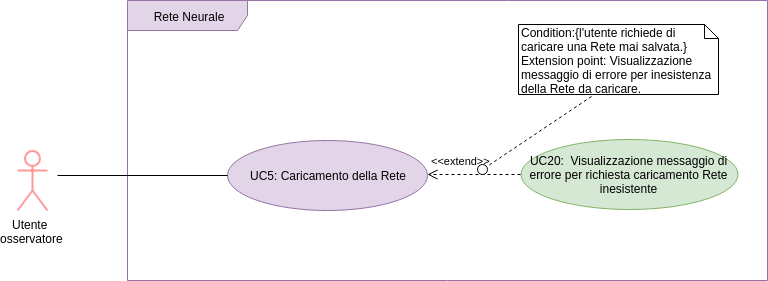
\includegraphics[width=1\linewidth]{./image/uc1.png}
	\caption{UC0\_g: Operazioni utente - Visione generale interfacciamento con la Rete neurale (Caricamento formato dati).}
	\label{UC0_g: Operazioni utente - Visione generale interfacciamento con la Rete neurale (Caricamento formato dati).}
\end{figure}
\noindent

\begin{itemize}
\item \textbf{Descrizione}: Il sistema permette all'utente di poter caricare i dati su cui effettuare l'analisi usando formato csv o txt;
\item \textbf{Attori}: Utente osservatore;
\item \textbf{Precondizione}: La Rete neurale \`e in attesa che l'utente effettui l'operazione di caricamento del file di dati;
\item \textbf{Postcondizione}: L'utente ha potuto caricare il file di dati di suo interesse nel formato idoneo;
\item \textbf{Scenario principale}:
\begin{enumerate}
\item L'utente pu\`o effettuare il caricamento di un formato di dati csv (UC2);
\item L'utente pu\`o effettuare il caricamento di un formato di dati txt (UC3).
\end{enumerate}
\item \textbf{Estensioni}:
\begin{enumerate}
\item Il browser in uso dall'utente non supporta lo standard HTML5. Viene ritornato un messaggio esplicativo che indica l'impossibilit\`a di terminare l'operazione (UC9);
\item L'utente ha effettuato il caricamento di un formato di dati non conforme al formato csv o txt.  Viene ritornato un messaggio esplicativo che indica l'impossibilit\`a di terminare l'operazione (UC10).
\end{enumerate}
\end{itemize}


\textbf{UC2: Caricamento formato dati CSV}\mbox{}
\label{UC2: Caricamento formato dati CSV}
\begin{itemize}
\item \textbf{Descrizione}: Il sistema permette all'utente di poter caricare i dati su cui effettuare l'analisi usando formato csv;
\item \textbf{Attori}: Utente osservatore;
\item \textbf{Precondizione}: La Rete neurale \`e in attesa che l'utente effettui l'operazione di caricamento del file di dati;
\item \textbf{Postcondizione}: L'utente ha potuto caricare il file di dati di suo interesse nel formato csv;
\item \textbf{Scenario principale}:
\begin{enumerate}
\item L'utente sceglie il file di dati che vuole caricare nella Rete;
\item L'utente confermare l'operazione.
\end{enumerate}
\end{itemize}


\textbf{UC3: Caricamento formato dati TXT}\mbox{}
\label{UC3: Caricamento formato dati TXT}
\begin{itemize}
\item \textbf{Descrizione}: Il sistema permette all'utente di poter caricare i dati su cui effettuare l'analisi usando formato txt;
\item \textbf{Attori}: Utente osservatore;
\item \textbf{Precondizione}: La Rete neurale \`e in attesa che l'utente effettui l'operazione di caricamento del file di dati;
\item \textbf{Postcondizione}: L'utente ha potuto caricare il file di dati di suo interesse nel formato txt;
\item \textbf{Scenario principale}:
\begin{enumerate}
\item L'utente sceglie il file di dati che vuole caricare nella Rete;
\item L'utente confermare l'operazione.
\end{enumerate}
\end{itemize}


\textbf{UC12: Visualizzazione messaggio di errore di mancata idoneità del browser in uso}\mbox{}
\label{UC12: Visualizzazione messaggio di errore di mancata idoneita del browser in uso}
\begin{itemize}
\item \textbf{Descrizione}: Il file nel formato corretto viene caricato nel sistema, che non \`e in grado di preocessare alcuna informazione in quanto il browser in uso dall'utente non supporta lo standard di markup HTML5;
\item \textbf{Attori}: Utente osservatore;
\item \textbf{Precondizione}: L'utente non ha ancora caricato il file nella Rete;
\item \textbf{Postcondizione}: Il sistema produce un messaggio d'errore per l'utente; con il quale quest'ultimo viene informato nella non conformit\`a del browser in uso agli standard minimi richiesti per portare a termine l'operazione di caricamento del file nella Rete con successo;
\item \textbf{Scenario principale}: Il file scelto dall'utente viene caricato all'interno della Rete.
\end{itemize}


\textbf{UC13: Visualizzazione messaggio di errore per formato di dati non coerente con le aspettative}\mbox{}
\label{UC13: Visualizzazione messaggio di errore per formato di dati non coerente con le aspettative}
\begin{itemize}
\item \textbf{Descrizione}:Il file nel che viene caricato nella rete non \`e del formato richiesto corretto;
\item \textbf{Attori}: Utente osservatore;
\item \textbf{Precondizione}: L'utente non ha ancora caricato il file nella Rete;
\item \textbf{Postcondizione}: Il sistema produce un messaggio d'errore per l'utente; con il quale quest'ultimo viene informato nella non conformit\`a del del formato di dati scelto;
\item \textbf{Scenario principale}: Il file viene caricato all'interno della Rete.
\end{itemize}
 
\subparagraph{UC4: Salvataggio della Rete}\mbox{} 
\label{UC4: Salvataggio della Rete}
\noindent
\begin{figure}[H]
\centering
	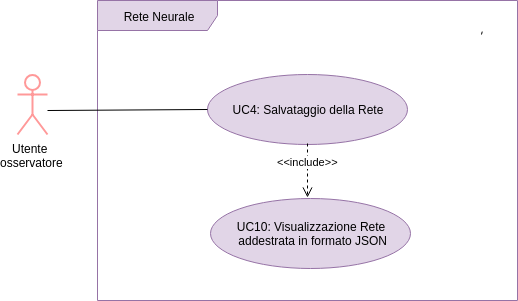
\includegraphics[width=0.80\linewidth]{./image/uc4.png}
	\caption{UC0\_g: Operazioni utente - Visione generale interfacciamento con la Rete neurale (Salvataggio della Rete).}
	\label{UC0_g: Operazioni utente - Visione generale interfacciamento con la Rete neurale (Salvataggio della Rete).}
\end{figure}
\noindent

\begin{itemize}
\item \textbf{Descrizione}: L'utente richiede che i dati caricati all'interno della Rete vengano salvati nello stato in cui si trovano;
\item \textbf{Attori}: Utente osservatore;
\item \textbf{Precondizione}: : L'utente ha caricato un file dati nella Rete e quest'ultima ne ha provveduto all'addestramento;
\item \textbf{Postcondizione}: L'utente ha gestito i dati caricati all'interno della Rete in modo da salvare la Rete;
\item \textbf{Scenario principale}:
\begin{enumerate}
\item L'utente effettua l'operazione di salvataggio della Rete.
\end{enumerate}
\end{itemize}

\subparagraph{UC10: Visualizzazione Rete addestrata in formato JSON}\mbox{}
\label{UC10: Visualizzazione Rete addestrata in formato JSON}
\noindent
\begin{itemize}
\item \textbf{Descrizione}: L'utente visualizza in formato JSON i dati della Rete sottoposti ad addestramento;
\item \textbf{Attori}: Utente osservatore;
\item \textbf{Precondizione}: L'utente ha effettuato il salvataggio della Rete;
\item \textbf{Postcondizione}: L'utente ha visualizzato la Rete salvata tradotta in formato JSON all'interno della textarea riservata dell'applicativo
\item \textbf{Scenario principale}:
\begin{enumerate}
\item L'utente visualizza i dati addestrati in formato JSON.
\end{enumerate}
\end{itemize}



\textbf{UC5: Caricamento della Rete}\mbox{}
\label{UC5: Caricamento della Rete}
\noindent
\begin{figure}[H]
\centering
	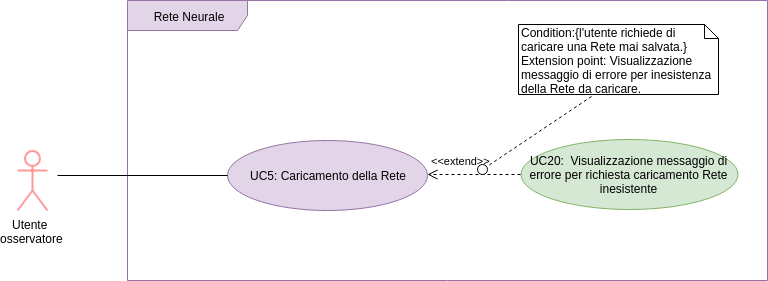
\includegraphics[width=1\linewidth]{./image/uc5.png}
	\caption{UC0\_g: Operazioni utente - Visione generale interfacciamento con la Rete neurale (Caricamento della Rete).}
	\label{UC0_g: Operazioni utente - Visione generale interfacciamento con la Rete neurale (Caricamento della Rete).}
\end{figure}
\noindent
\begin{itemize}
\item \textbf{Descrizione}: L'utente richiede che la Rete salvata precedentemente venga ricaricata e preparata all'uso nella Rete;
\item \textbf{Attori}: Utente osservatore;
\item \textbf{Precondizione}: L'utente ha salvato una Rete precedentemente
\item \textbf{Postcondizione}: L'utente ha gestito i dati caricati all'interno della Rete in modo da ricaricare una Rete precedentemente salvata;
\item \textbf{Scenario principale}:
\begin{enumerate}
\item L'utente richiede l'operazione di caricamento della Rete precedente salvata.
\end{enumerate}
\item \textbf{Estensioni}:
\begin{enumerate}
\item L'utente ha richiesto il caricamento di una Rete mai precedentemente salvata. Viene ritornato un messaggio esplicativo che indica l'impossibilit\`a di terminare l'operazione (UC14).
\end{enumerate}
\end{itemize}

\textbf{UC14: Visualizzazione messaggio di errore per richiesta caricamento Rete inesistente}\mbox{}
\label{UC14: Visualizzazione messaggio di errore per richiesta caricamento Rete inesistente}
\noindent
\begin{itemize}
\item \textbf{Descrizione}: L'utente visualizza un messaggio di errore nel caso in cui abbia richiesto il caricamento di una Rete quando non non ne \`e ancora stata salvata nessuna;
\item \textbf{Attori}: Utente osservatore;
\item \textbf{Precondizione}: L'utente ha richiesto il caricamento dei dati della Rete precedente;
\item \textbf{Postcondizione}: Il sistema ha fornito all'utente la visualizzazione di un messaggio di errore che indica l'inesistenza della Rete da caricare richiesta.
\item \textbf{Scenario principale}:
\begin{enumerate}
\item All'utente viene indicato l'errore.
\end{enumerate}
\end{itemize}


\subparagraph{UC6: Visualizzazione batch di dati inseriti}\mbox{}
\label{UC6: Visualizzazione batch di dati inseriti}
\noindent
\begin{figure}[H]
\centering
	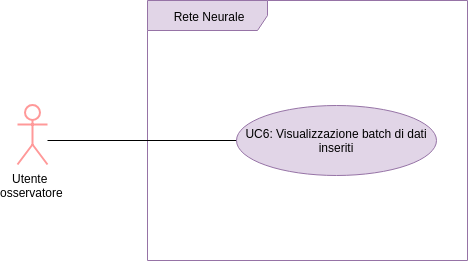
\includegraphics[width=0.80\linewidth]{./image/uc6.png}
	\caption{UC0\_g: Operazioni utente - Visione generale interfacciamento con la Rete neurale (Visualizzazione batch di dati inseriti).}
	\label{UC0_g: Operazioni utente - Visione generale interfacciamento con la Rete neurale (Visualizzazione batch di dati inseriti).}
\end{figure}
\noindent
\begin{itemize}
\item \textbf{Descrizione}: L'utente visualizza i dati caricati nella Rete all'interno di una textarea riservata, all'interno della pagina web dell'applicativo; e ne pu\`o ottenere un maggior dettaglio visualizzando gli stessi su una pagina web riservata, in cui vengono evidenziati i significati dei dati mostrati;
\item \textbf{Attori}: Utente osservatore;
\item \textbf{Precondizione}: L'utente ha  effettuato il caricamento dei dati nella Rete in uno dei formati idonei;
\item \textbf{Postcondizione}: L'utente visualizza il batch di dati caricati nella Rete;
\item \textbf{Scenario principale}:
\begin{enumerate}
\item L'utente visualizza i dati caricati nella Rete all'interno della pagina web dell'applicativo stesso (UC6.1);
\item L'utente visualizza i dati caricati nella Rete su una pagina web a parte (UC6.2).
\end{enumerate}
\end{itemize}

\textbf{UC6.1: Visualizzazione dei dati caricati all'interno della pagina web riservata all'applicativo}\mbox{}
\label{UC6.1: Visualizzazione dei dati caricati all'interno della pagina web riservata all'applicativo}
\noindent
\begin{itemize}
\item \textbf{Descrizione}: L'utente visualizza i dati caricati nella Rete all'interno di una textarea riservata, all'interno della pagina web dell'applicativo, che ha il compito di tenere traccia di tutte le operazioni svolte nella Rete;
\item \textbf{Attori}: Utente osservatore;
\item \textbf{Precondizione}: L'utente ha  effettuato il caricamento dei dati nella Rete in uno dei formati idonei;
\item \textbf{Postcondizione}: L'utente ha visualizzato all'interno della textarea i vettori di dati caricati nella Rete;
\item \textbf{Scenario principale}:
\begin{enumerate}
\item L'utente visualizza i dati caricati nella Rete all'interno della textarea dell'applicativo della Rete prima che il sistema proceda con l'addestramento
\end{enumerate}
\end{itemize}

\textbf{UC6.2: Visualizzazione dei dati caricati all'interno della Rete su pagina web a parte}\mbox{}
\label{UC6.2: Visualizzazione dei dati caricati all'interno della Rete su pagina web a parte}
\noindent
\begin{itemize}
\item \textbf{Descrizione}: L'utente visualizza i dati caricati nella Rete su una pagina web riservata ad adempiere tale mansione. I dati caricati vengono presentati con indicazione del numero di test e di domanda a cui ognuno fa capo, cos\`e che all'utente risulti pi\`u agevole effettuare una veloce osservazione sugli stessi.
\item \textbf{Attori}: Utente osservatore;
\item \textbf{Precondizione}: L'utente ha  effettuato il caricamento dei dati nella Rete in uno dei formati idonei;
\item \textbf{Postcondizione}: L'utente ha visualizzato all'interno di una pagina web riservata i vettori di dati caricati nella Rete;
\item \textbf{Scenario principale}:
\begin{enumerate}
\item L'utente visualizza i dati caricati nella Rete all'interno di una pagina web reindirizzata dall'applicativo della Rete stessa.
\end{enumerate}
\end{itemize}

\subparagraph{UC7: Modifica architettura della Rete}\mbox{}
\label{UC7: Modifica architettura della Rete}
\noindent
\begin{figure}[H]
\centering
	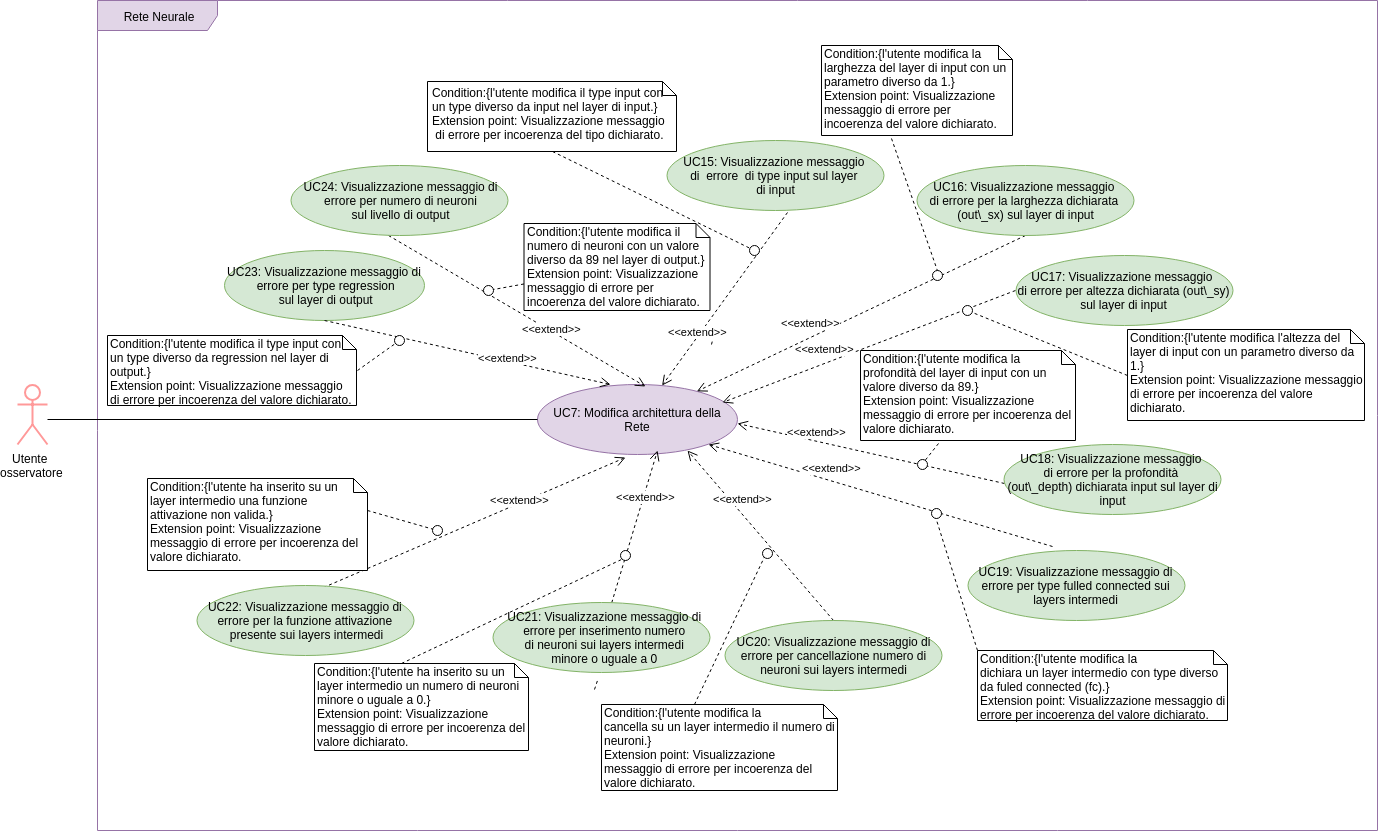
\includegraphics[width=1.10\linewidth]{./image/uc7.png}
	\caption{UC0\_g: Operazioni utente - Visione generale interfacciamento con la Rete neurale (Modifica architettura della Rete).}
	\label{UC0_g: Operazioni utente - Visione generale interfacciamento con la Rete neurale (Modifica architettura della Rete).}
\end{figure}
\noindent
\begin{itemize}
\item \textbf{Descrizione}: L'utente ha la possibilit\`a di riconfigurare l'architettura della Rete neurale. Esso pu\`o procedere a modificare il numero di neuroni per layer, impostare dei nuovi layers, eliminare i layers intermedi esistenti, modificare/eliminare la funzione attivazione e ridefinire i parametri del trainer della Rete;
\item \textbf{Attori}: Utente osservatore;
\item \textbf{Precondizione}: L'utente non ha ancora effettuato alcuna operazione e la Rete desiderata ancora non esiste;
\item \textbf{Postcondizione}: L'utente ha provveduto a configurare la Rete in base alle proprie necessit\`a;
\item \textbf{Scenario principale}:
\begin{enumerate}
\item L'utente ha aggiunto un nuovo layer intermedio nella Rete (UC7.1);
\item L'utente ha eliminato un layer intermedio esistente nella Rete (UC7.2);
\item L'utente ha modificato un layer intermedio (UC7.3);
\item L'utente ha modificato i parametri del trainer della Rete (UC7.4);
\item L'utente conferma l'operazione di modifica della Rete (UC7.5);
\end{enumerate}
\item \textbf{Estensioni}:
\begin{enumerate}
\item L'utente ha tentato di modificare il type input sul layer di input della Rete. Viene ritornato un messaggio esplicativo che indica l'impossibilit\`a di terminare l'operazione (UC15);
\item L'utente ha tentato di modificare la larghezza dichiarata (out\_sx) sul layer di input della Rete. Viene ritornato un messaggio esplicativo che indica l'impossibilit\`a di terminare l'operazione (UC16);
\item L'utente ha tentato di modificare l'altezza dichiarata (out\_sy) sul layer di input della Rete. Viene ritornato un messaggio esplicativo che indica l'impossibilit\`a di terminare l'operazione (UC17);
\item L'utente ha tentato di modificare la profondit\`a dichiarata (out\_depth) sul layer di input della Rete. Viene ritornato un messaggio esplicativo che indica l'impossibilit\`a di terminare l'operazione (UC18);
\item L'utente ha tentato di modificare il tipo di connessione fulled connected su un layer intermedio della Rete. Viene ritornato un messaggio esplicativo che indica l'impossibilit\`a di terminare l'operazione (UC19);
\item L'utente ha tentato di cancellare il numero di neuroni presenti su un layer intermedio della Rete. Viene ritornato un messaggio esplicativo che indica l'impossibilit\`a di terminare l'operazione (UC20);
\item L'utente ha tentato di inserire un numero di neuroni presenti su un layer intermedio della Rete minore o uguale a 0. Viene ritornato un messaggio esplicativo che indica l'impossibilit\`a di terminare l'operazione (UC21);
\item L'utente ha tentato di modificare la funzione di attivazione su un layer intermedio della Rete, con una dichiarazione di funzione non valida. Viene ritornato un messaggio esplicativo che indica l'impossibilit\`a di terminare l'operazione (UC22);
\item L'utente ha tentato di modificare il tipo regressione presente sul layer di output della Rete. Viene ritornato un messaggio esplicativo che indica l'impossibilit\`a di terminare l'operazione (UC23);
\item L'utente ha tentato di modificare il numero di neuroni presente sul layer di output della Rete. Viene ritornato un messaggio esplicativo che indica l'impossibilit\`a di terminare l'operazione (UC24).
\end{enumerate}
\end{itemize}

\textbf{UC7.1: Aggiunta layer intermedio}
\label{UC7.1: Aggiunta layer intemrdio}
\noindent
\begin{itemize}
\item \textbf{Descrizione}: L'utente ha la possibilit\`a di riconfigurare l'architettura della Rete neurale. Esso pu\`o procedere ad aggiungere un layer intermedio nella Rete;
\item \textbf{Attori}: Utente osservatore;
\item \textbf{Precondizione}: L'utente non ha ancora effettuato alcuna operazione e la Rete desiderata ancora non esiste;
\item \textbf{Postcondizione}: L'utente ha provveduto a configurare la Rete in base alle proprie necessit\`a aggiungendo un nuovo layer intermedio;
\item \textbf{Scenario principale}:
\begin{enumerate}
\item L'utente ha aggiunto un layer intermedio alla Rete:
\begin{enumerate}
\item L'utente effettua l'inserimento del parametro di tipo;
\item L'utente effettua l'inserimento del numero di neuroni;
\item L'utente pu\`o indicare o meno la funzione attivazione;
\item L'utente conferma l'operazione di modifica della Rete.
\end{enumerate}
\end{enumerate}
\end{itemize}

\textbf{UC7.2: Eliminazione layer intermedio esistente}
\label{UC7.2: Eliminazione layer intermedio esistente}
\noindent
\begin{itemize}
\item \textbf{Descrizione}: L'utente ha la possibilit\`a di riconfigurare l'architettura della Rete neurale. Esso pu\`o procedere a eliminare un layer intermedio presente nella Rete;
\item \textbf{Attori}: Utente osservatore;
\item \textbf{Precondizione}: L'utente non ha ancora effettuato alcuna operazione e la Rete desiderata ancora non esiste;
\item \textbf{Postcondizione}: L'utente ha provveduto a configurare la Rete in base alle proprie necessit\`a eliminando un layer intermedio;
\item \textbf{Scenario principale}:
\begin{enumerate}
\item L'utente ha eliminato un layer intermedio esistente nella Rete:
\begin{enumerate}
\item L'utente elimina il parametro di tipo;
\item L'utente elimina il numero di numero di neuroni;
\item L'utente elimina se presente la funzione attivazione;
\item L'utente conferma l'operazione di modifica della Rete.
\end{enumerate}
\end{enumerate}
\end{itemize}

\textbf{UC7.3: Modifica layer intermedio esistente}
\label{UC7.3: Modifica layer intermedio esistente}
\noindent
\begin{itemize}
\item \textbf{Descrizione}: L'utente ha la possibilit\`a di modificare un layer intermedio presente nella Rete
\item \textbf{Attori}: Utente osservatore;
\item \textbf{Precondizione}: L'utente non ha ancora effettuato alcuna operazione e la Rete desiderata ancora non esiste;
\item \textbf{Postcondizione}: L'utente ha provveduto a configurare la Rete in base alle proprie necessit\`a 
provvedendo a ridefinire il contenuto di un layer intermedio;
\item \textbf{Scenario principale}:
\begin{enumerate}
\item L'utente ha ridefinito un layer intermedio presente nella Rete:
\begin{enumerate}
\item L'utente pu\`o modificare il numero di neuroni presenti nella Rete;
\item L'utente pu\`o modificare il parametro modificare/aggiungere/eliminare la funzione attivazione;
\item L'utente conferma l'operazione di modifica della Rete.
\end{enumerate}
\end{enumerate}
\end{itemize}


\textbf{UC7.4: Modifica di trainer}
\label{UC7.4: Modifica di trainer}
\noindent
\begin{itemize}
\item \textbf{Descrizione}: L'utente ha la possibilit\`a di configurare la dichiarazione del trainer della Rete
\item \textbf{Attori}: Utente osservatore;
\item \textbf{Precondizione}: L'utente non ha ancora effettuato alcuna operazione e la Rete desiderata ancora non esiste;
\item \textbf{Postcondizione}: L'utente ha provveduto a configurare la Rete in base alle proprie necessit\`a definendo il trainer;
\item \textbf{Scenario principale}:
\begin{enumerate}
\item L'utente ha configurato il trainer della Rete:
\begin{enumerate}
\item L'utente pu\`o modificare il parametro di learning\_rate;
\item L'utente pu\`o modificare il parametro momentum;
\item L'utente pu\`o modificare il parametro batch\_size;
\item L'utente pu\`o modificare il parametro l2\_decay;
\item L'utente conferma l'operazione di modifica della Rete.
\end{enumerate}
\end{enumerate}
\end{itemize}


\textbf{UC15: Visualizzazione messaggio di errore di type input sul layer di input}
\label{UC15: Visualizzazione messaggio di errore di type input sul layer di input}
\noindent
\begin{itemize}
\item \textbf{Descrizione}: L'utente visualizza un messaggio di errore nel caso in cui abbia modificato nel layer di input il tipo dello stesso;
\item \textbf{Attori}: Utente osservatore;
\item \textbf{Precondizione}: L'utente ha fornito un tipo nel nel layer di input
\item \textbf{Postcondizione}: Il sistema ha fornito all'utente la visualizzazione di un messaggio di errore che indica la incompatibilit\`a del tipo richiesto con la natura della Rete.
\item \textbf{Scenario principale}:
\begin{enumerate}
\item All'utente viene indicato l'errore con l'indicazione della correzione necessaria per il corretto funzionamento dalla Rete.
\end{enumerate}
\end{itemize}

\textbf{UC16: Visualizzazione messaggio di errore per la larghezza dichiarata (out\_sx) sul layer di input}
\label{UC16: Visualizzazione messaggio di errore per la larghezza dichiarata sul layer di input}
\noindent
\begin{itemize}
\item \textbf{Descrizione}: L'utente visualizza un messaggio di errore nel caso in cui abbia modificato nel layer di input la larghezza dichiarata;
\item \textbf{Attori}: Utente osservatore;
\item \textbf{Precondizione}: L'utente ha fornito la dimensione della larghezza della componente base della Rete Vol;
\item \textbf{Postcondizione}: Il sistema ha fornito all'utente la visualizzazione di un messaggio di errore che indica la incompatibilit\`a del della dimensione richiesta con la natura della Rete.
\item \textbf{Scenario principale}:
\begin{enumerate}
\item All'utente viene indicato l'errore con l'indicazione della correzione necessaria per il corretto funzionamento dalla Rete.
\end{enumerate}
\end{itemize}

\textbf{UC17: Visualizzazione messaggio di errore per altezza dichiarata (out\_sy) sul layer di input}
\label{UC17: Visualizzazione messaggio di errore per altezza dichiarata sul layer di input}
\noindent
\begin{itemize}
\item \textbf{Descrizione}: L'utente visualizza un messaggio di errore nel caso in cui abbia modificato nel layer di input l'altezza dichiarata;
\item \textbf{Attori}: Utente osservatore;
\item \textbf{Precondizione}: L'utente ha fornito la dimensione dell'altezza della componente base della Rete Vol;
\item \textbf{Postcondizione}: Il sistema ha fornito all'utente la visualizzazione di un messaggio di errore che indica la incompatibilit\`a del della dimensione richiesta con la natura della Rete.
\item \textbf{Scenario principale}:
\begin{enumerate}
\item All'utente viene indicato l'errore con l'indicazione della correzione necessaria per il corretto funzionamento dalla Rete.
\end{enumerate}
\end{itemize}


\textbf{UC18: Visualizzazione messaggio di errore per la profondit\`a (out\_depth) dichiarata input sul layer di input}
\label{UC18: Visualizzazione messaggio di errore per la profondita dichiarata input sul layer di input}
\noindent
\begin{itemize}
\item \textbf{Descrizione}: L'utente visualizza un messaggio di errore nel caso in cui abbia modificato nel layer di input la profondit\`a dichiarata;
\item \textbf{Attori}: Utente osservatore;
\item \textbf{Precondizione}: L'utente ha fornito la dimensione della profondit\`a della componente base della Rete Vol;
\item \textbf{Postcondizione}: Il sistema ha fornito all'utente la visualizzazione di un messaggio di errore che indica la incompatibilit\`a del della dimensione richiesta con la natura della Rete.
\item \textbf{Scenario principale}:
\begin{enumerate}
\item All'utente viene indicato l'errore con l'indicazione della correzione necessaria per il corretto funzionamento dalla Rete.
\end{enumerate}
\end{itemize}


\textbf{UC19: Visualizzazione messaggio di errore per type fulled connected sui layers intermedi}
\label{UC19: Visualizzazione messaggio di errore per type fulled connected sui layers intermedi}
\noindent
\begin{itemize}
\item \textbf{Descrizione}: L'utente visualizza un messaggio di errore nel caso in cui abbia inserito in uno dei layers intermedi un tipo diverso da fulled connected;
\item \textbf{Attori}: Utente osservatore;
\item \textbf{Precondizione}: L'utente ha fornito il tipo in un layer intermedio;
\item \textbf{Postcondizione}: Il sistema ha fornito all'utente la visualizzazione di un messaggio di errore che indica la incompatibilit\`a del tipo richiesto con la natura della Rete.
\item \textbf{Scenario principale}:
\begin{enumerate}
\item All'utente viene indicato l'errore con l'indicazione della correzione necessaria per il corretto funzionamento dalla Rete.
\end{enumerate}
\end{itemize}


\textbf{UC20: Visualizzazione messaggio di errore per cancellazione numero di neuroni sui layers intermedi}
\label{UC20: Visualizzazione messaggio di errore per cancellazione numero di neuroni sui layers intermedi}
\noindent
\begin{itemize}
\item \textbf{Descrizione}: L'utente visualizza un messaggio di errore nel caso in cui effettuato la cancellazione in uno dei layers intermedi del numero di neuroni presenti;
\item \textbf{Attori}: Utente osservatore;
\item \textbf{Precondizione}: L'utente ha eliminato il numero di neuroni da un layer intermedio;
\item \textbf{Postcondizione}: Il sistema ha fornito all'utente la visualizzazione di un messaggio di errore che indica la incompatibilit\`a dell'operazione richiesta con la natura della Rete.
\item \textbf{Scenario principale}:
\begin{enumerate}
\item All'utente viene indicato l'errore con l'indicazione della correzione necessaria per il corretto funzionamento dalla Rete.
\end{enumerate}
\end{itemize}

\textbf{UC21: Visualizzazione messaggio di errore per inserimento numero di neuroni sui layers intermedi minore o uguale a 0}
\label{UC21: Visualizzazione messaggio di errore per inserimento numero di neuroni sui layers intermedi minore o uguale a 0}
\noindent
\begin{itemize}
\item \textbf{Descrizione}: L'utente visualizza un messaggio di errore nel caso abbia inserito/modificato il numero di neuroni presenti in un layer intermedio con un valore minore o uguale a 0;
\item \textbf{Attori}: Utente osservatore;
\item \textbf{Precondizione}: L'utente ha inserito il numero di neuroni in un layer intermedio;
\item \textbf{Postcondizione}: Il sistema ha fornito all'utente la visualizzazione di un messaggio di errore che indica la incompatibilit\`a del valore definito con la natura della Rete.
\item \textbf{Scenario principale}:
\begin{enumerate}
\item All'utente viene indicato l'errore con l'indicazione della correzione necessaria per il corretto funzionamento dalla Rete.
\end{enumerate}
\end{itemize}


\textbf{UC22: Visualizzazione messaggio di errore per la funzione attivazione presente sui layers intermedi}
\label{UC22: Visualizzazione messaggio di errore per la funzione attivazione presente sui layers intermedi}
\noindent
\begin{itemize}
\item \textbf{Descrizione}: L'utente visualizza un messaggio di errore nel caso abbia inserito/modificato  la funzione di attivazione su un layer intermedio con parametro diverso da uno dei desiderati.
\item \textbf{Attori}: Utente osservatore;
\item \textbf{Precondizione}: L'utente ha inserito una funzione attivazione in un layer intermedio;
\item \textbf{Postcondizione}: Il sistema ha fornito all'utente la visualizzazione di un messaggio di errore che indica l'inesistenza della funzione attivazione richiesta per la Rete.
\item \textbf{Scenario principale}:
\begin{enumerate}
\item All'utente viene indicato l'errore con l'indicazione della correzione necessaria per il corretto funzionamento dalla Rete.
\end{enumerate}
\end{itemize}

\textbf{UC23: Visualizzazione messaggio di errore per type regression sul layer di output}
\label{UC23: Visualizzazione messaggio di errore per type regression sul layer di output}
\noindent
\begin{itemize}
\item \textbf{Descrizione}: L'utente visualizza un messaggio di errore nel caso abbia modificato il tipo dichiarato nel layer di output
\item \textbf{Attori}: Utente osservatore;
\item \textbf{Precondizione}: L'utente ha modificato il tipo presente nel layer di output;
\item \textbf{Postcondizione}: Il sistema ha fornito all'utente la visualizzazione di un messaggio di errore che indica l'incompatibilit\`a del valore del tipo richiesto con la natura della Rete;
\item \textbf{Scenario principale}:
\begin{enumerate}
\item All'utente viene indicato l'errore con l'indicazione della correzione necessaria per il corretto funzionamento dalla Rete.
\end{enumerate}
\end{itemize}

\textbf{UC24: Visualizzazione messaggio di errore per numero di neuroni sul livello di output}
\label{UC24: Visualizzazione messaggio di errore per numero di neuroni sul livello di output}
\noindent
\begin{itemize}
\item \textbf{Descrizione}: L'utente visualizza un messaggio di errore nel caso abbia modificato il numero di neuroni dichiarati nel layer di output
\item \textbf{Attori}: Utente osservatore;
\item \textbf{Precondizione}: L'utente ha modificato il numero di neuroni presenti nel layer di output;
\item \textbf{Postcondizione}: Il sistema ha fornito all'utente la visualizzazione di un messaggio di errore che indica  l'incompatibilit\`a del tipo di neuroni richiesti con la natura della Rete;
\item \textbf{Scenario principale}:
\begin{enumerate}
\item All'utente viene indicato l'errore con l'indicazione della correzione necessaria per il corretto funzionamento dalla Rete.
\end{enumerate}
\end{itemize}

\subparagraph{UC8: Gestione inserimento parametri di previsione}\mbox{}
\label{UC8: Gestione inserimento parametri di previsione}
\noindent
\begin{itemize}
\item \textbf{Descrizione}: L'utente inserisce i parametri necessari per effettuare previsione sui dati addestrati della Rete;
\item \textbf{Attori}: Utente osservatore;
\item \textbf{Precondizione}: La Rete \`e addestrata con i dati caricati dall'utente;
\item \textbf{Postcondizione}: L'utente ha ottenuto la previsione sui dati addestrati in base ai parametri passati in input alla Rete;
\item \textbf{Scenario principale}:
\begin{enumerate}
\item  L'utente ha inserito i parametri necessari per effettuare una clusterizzazione sui dati, una volta predetti dall'applicativo (UC8.1);
\item L'utente ha selezionato per ogni domanda una delle risposte, tra quelle concesse, in modo da generare un vettore previsione su cui effettuare con questi una previsione sui dati addestrati dalla Rete (UC8.2);
\item L'utente ha confermato le operazioni dando il via al calcolo dei risultati di previsione (UC8.3).
\end{enumerate}
\textbf{Estensioni:}
\begin{enumerate}
\item L'utente ha inserito per uno o pi\`u dei parametri di clusterizzazione un valore stringa. Viene ritornato un messaggio esplicativo che indica l'impossibilit\`a di terminare l'operazione (UC25);
\item L'utente ha inserito per uno o pi\`u dei parametri di clusterizzazione un valore vuoto. Viene ritornato un messaggio esplicativo che indica l'impossibilit\`a di terminare l'operazione (UC26);
\item L'utente ha inserito per uno o pi\`u dei parametri di clusterizzazione un numero negativo. Viene ritornato un messaggio esplicativo che indica l'impossibilit\`a di terminare l'operazione (UC27);
\item L'utente ha inserito per uno o pi\`u dei parametri di clusterizzazione un numero superiore a 255. Viene ritornato un messaggio esplicativo che indica l'impossibilit\`a di terminare l'operazione (UC28).
\end{enumerate}
\end{itemize}

\subparagraph{UC9: Visualizzazione risultati della Rete}\mbox{}
\label{UC9: Visualizzazione risultati della Rete}
\noindent
\begin{itemize}
\item \textbf{Descrizione}: L'utente visualizza i risultati ottenuti dalla Rete a seguito della richiesta di previsione sui dati addestrati della Rete;
\item \textbf{Attori}: Utente osservatore;
\item \textbf{Precondizione}: La Rete \`e addestrata e con richiesta di previsione pendente;
\item \textbf{Postcondizione}: L'utente ha visualizzato i risultati di previsione ottenuti dalla Rete; 
\item \textbf{Scenario principale}:
\begin{enumerate}
\item Visualizzazione nella textarea riservata dell'applicativo dei risultati di previsione ottenuti, espressi in termini numerici su ogni domanda (UC9.1);
\item Visualizzazione nella textarea riservata dell'applicativo dei risultati di previsione ottenuti, espressi in codice rgb su ogni domanda (UC9.2);
\item Visualizzazione nella textarea riservata dell'applicativo dei cluster delle domande generati sulla base dei parametri di clusterizzazione passati in input e applicati alle previsioni espresse in codice rgb (UC9.3);
\item Visualizzazione generale, mediante tecnologia canvas, dei risultati delle previsioni, espressi in termini rgb su ogni domanda (UC9.4).
\end{enumerate}
\end{itemize}

\textbf{UC9.4: Visualizzazione dei risultati di previsione mediante canvas}\mbox{}\\\\
\label{UC9.4: Visualizzazione dei risultati di previsione mediante canvas}
\noindent
\begin{itemize}
\item \textbf{Descrizione}: L'utente visualizza i risultati ottenuti dalla Rete, mediante canvas applicati alle previsioni espresse in termini rgb, a seguito della richiesta di previsione sui dati addestrati della Rete;
\item \textbf{Attori}: Utente osservatore;
\item \textbf{Precondizione}: La Rete \`e addestrata e con richiesta di previsione pendente;
\item \textbf{Postcondizione}: L'utente ha visualizzato i risultati di previsione ottenuti dalla Rete rappresentato per mezzo di canvas; 
\item \textbf{Scenario principale}:
\begin{enumerate}
\item Visualizzazione di un quadrato per ogni domanda in analisi con gradazione verde, bianco, rosso; sulla base del risultato di previsione ottenuto a seguito dell'addestramento della Rete e del vettore previsione inoltrato in input.
\item Visualizzazione di dettaglio, mediante tecnologia canvas, della previsione ottenuta (UC9.4.1). 
\end{enumerate}
\end{itemize}

\textbf{UC9.4.1: Visualizzazione dei risultati di previsione in dettaglio mediante canvas}\mbox{}\\\\
\label{UC9.4.1: Visualizzazione dei risultati di previsione in dettaglio mediante canvas}
\noindent
\begin{itemize}
\item \textbf{Descrizione}: L'utente visualizza i risultati ottenuti dalla Rete, mediante canvas applicata alle previsioni espresse in termini rgb su un vettore previsione che pone come domanda corretta solo la domanda in esame;
\item \textbf{Attori}: Utente osservatore;
\item \textbf{Precondizione}: La Rete ha effettuato previsione sui dati;
\item \textbf{Postcondizione}: L'utente ha visualizzato i risultati di previsione di dettaglio ottenuti dalla Rete rappresentato per mezzo di canvas; 
\item \textbf{Scenario principale}:
\begin{enumerate}
\item Visualizzazione di un quadrato tanti quante sono le domande, per ogni domanda in analisi, con gradazione verde, bianco, rosso. La gradazione \`e calcolata sul risultato di previsione ottenuto a seguito dell'addestramento della Rete e del vettore previsione che pone corretta la domanda in esame e sbagliate tutte le rimanenti.
\end{enumerate}
\end{itemize}

\subparagraph{UC11: Pulizia della textarea riservata a visualizzare lo storico dell'applicativo}\mbox{}
\label{Pulizia della textarea riservata a visualizzare lo storico dell'applicativo}
\noindent
\begin{itemize}
\item \textbf{Descrizione}: L'utente effettua la cancellazione dello storico in visualizzazione della textarea riservata;
\item \textbf{Attori}: Utente osservatore;
\item \textbf{Precondizione}: L'utente ha effettuato nella Rete alcune o anche nessuna operazione;
\item \textbf{Postcondizione}: L'utente visualizza la textarea pulita dallo storico delle operazioni effettuate dalla Rete;
\item \textbf{Scenario principale}:
\begin{enumerate}
\item L'utente visualizza l'area di lavoro priva di informazioni sui dati elaborati fino a quel momento.
\end{enumerate}
\end{itemize}
